\documentclass[11pt, twoside]{report}   %11 point font
\usepackage[utf8]{inputenc}
\usepackage[a4paper, left=30mm, right=20mm, top=25mm, bottom=25mm]{geometry}

\usepackage{helvet}
\renewcommand{\familydefault}{\sfdefault}
%\usepackage{times}  %set Times New Roman as the font

% used for points after order numbers
\usepackage[titles]{tocloft}  %table of contents control and formatting
\makeatletter
\renewcommand*\@seccntformat[1]{\csname the#1\endcsname.\enspace}
\makeatother
\renewcommand{\cftchapaftersnum}{.} % zakomentować dla 'article'
\renewcommand{\cftsecaftersnum}{.}
\renewcommand{\cftsubsecaftersnum}{.}
\renewcommand{\cftsubsubsecaftersnum}{.}
\renewcommand{\cftparaaftersnum}{.}
\renewcommand{\cftsubparaaftersnum}{.}



\usepackage{fancyhdr}
\fancyhf{} % clear all header and footers
\renewcommand{\headrulewidth}{0pt} % remove the header rule
\fancyfoot[LE,RO]{\thepage} % Left side on Even pages; Right side on Odd pages
\pagestyle{fancy}
\fancypagestyle{plain}{%
  \fancyhf{}%
  \renewcommand{\headrulewidth}{0pt}%
  \fancyhf[lef,rof]{\thepage}%
}



\usepackage{graphicx}  %for images and plots
\usepackage{setspace}  %use this package to set linespacing as desired
\usepackage[explicit]{titlesec}  %title control and formatting
\usepackage[backend=bibtex, sorting=none, bibstyle=ieee]{biblatex}  %reference manager
\usepackage[bookmarks=true, hidelinks]{hyperref}
\usepackage[page]{appendix}  %for appendices
\usepackage{rotating}  %for rotated, landscape images
\usepackage[normalem]{ulem}  %for italicized text

\setlength{\parindent}{5mm}
\setlength{\parskip}{0mm}


\usepackage{csquotes}
\usepackage{multirow}
\usepackage{xcolor}
\usepackage{sectsty} % to change color of the section
\usepackage{listings}
\usepackage{acronym} 
\usepackage{amsmath}
\usepackage{threeparttable}

\usepackage{rotating} % to rotate the figure

\usepackage{pdfpages}

\usepackage{afterpage}
\newcommand\blankpage{%
    \null
    \thispagestyle{empty}%
    \newpage}

\definecolor{mGreen}{rgb}{0,0.6,0}
\definecolor{mGray}{rgb}{0.5,0.5,0.5}
\definecolor{mPurple}{rgb}{0.58,0,0.82}
\definecolor{backgroundColour}{rgb}{0.95,0.95,0.92}

\lstdefinestyle{CStyle}{
    backgroundcolor=\color{backgroundColour},   
    commentstyle=\color{mGreen},
    keywordstyle=\color{magenta},
    numberstyle=\tiny\color{mGray},
    stringstyle=\color{mPurple},
    basicstyle=\footnotesize,
    breakatwhitespace=false,         
    breaklines=true,                 
    captionpos=b,                    
    keepspaces=true,                 
    numbers=left,                    
    numbersep=5pt,                  
    showspaces=false,                
    showstringspaces=false,
    showtabs=false,                  
    tabsize=2,
    language=C
}

%%%%%%%%%%%%%%%%%%%%%%%%%%%%%%%%%%%
% Bibliography
%%%%%%%%%%%%%%%%%%%%%%%%%%%%%%%%%%%
%jabref look for it

%Add your bibliography file here
\bibliography{references}

% prevent certain fields in references from printing in bibliography
\AtEveryBibitem{\clearfield{issn}}
\AtEveryBibitem{\clearlist{issn}}

\AtEveryBibitem{\clearfield{language}}
\AtEveryBibitem{\clearlist{language}}

\AtEveryBibitem{\clearfield{doi}}
\AtEveryBibitem{\clearlist{doi}}

\AtEveryBibitem{\clearfield{url}}
\AtEveryBibitem{\clearlist{url}}

\AtEveryBibitem{%
  \ifentrytype{online}
    {}
    {\clearfield{urlyear}\clearfield{urlmonth}\clearfield{urlday}}}




%%%%%%%%%%%%%%%%%%%%%%%%%%%%%%%%%%%%%
% Table of Contents
%%%%%%%%%%%%%%%%%%%%%%%%%%%%%%%%%%%%%

% Format for Table of Contents
\renewcommand{\cftchapdotsep}{\cftdotsep}  %add dot separators
\renewcommand{\cftchapfont}{\bfseries}  %set title font weight
\renewcommand{\cftchappagefont}{}  %set page number font weight
\renewcommand{\cftchappresnum}{Chapter }
\renewcommand{\cftchapaftersnum}{:}
\renewcommand{\cftchapnumwidth}{5em}
\renewcommand{\cftchapafterpnum}{\vskip\baselineskip} %set correct spacing for entries in single space environment
\renewcommand{\cftsecafterpnum}{\vskip\baselineskip}  %set correct spacing for entries in single space environment
\renewcommand{\cftsubsecafterpnum}{\vskip\baselineskip} %set correct spacing for entries in single space environment
\renewcommand{\cftsubsubsecafterpnum}{\vskip\baselineskip} %set correct spacing for entries in single space environment

%format title font size and position (this also applys to list of figures and list of tables)
\titleformat{\chapter}[display]
{\normalfont\bfseries\filcenter}{\chaptertitlename\ \thechapter}{0pt}{\MakeUppercase{#1}}

\renewcommand\contentsname{Table of Contents}




\begin{document}
%\doublespacing  %set line spacing
\setstretch{1.15}

\includepdf{title_page.pdf}
\currentpdfbookmark{Title Page}{titlePage}  %add PDF bookmark for this page
\blankpage
Blebleble
\thispagestyle{empty}
\clearpage
\blankpage
\includepdf[pages={1, 2}]{declaration.pdf}


\begin{singlespace}
\tableofcontents
\end{singlespace}

\currentpdfbookmark{Table of Contents}{TOC}

\clearpage

% resume page numbering for rest of document
%\clearpage
%\pagenumbering{arabic}
%\setcounter{page}{1} % set the page number appropriately



% Adjust chapter title formatting
\titleformat{\chapter}[display]
{\normalfont\bfseries\filcenter}{\MakeUppercase\chaptertitlename\ \thechapter}{0pt}{\MakeUppercase{#1}}  %spacing between titles
\titlespacing*{\chapter}
  {0pt}{0pt}{30pt}	%controls vertical margins on title
  
% Adjust section title formatting
\titleformat{\section}{\normalfont\bfseries}{\thesection}{1em}{#1}

% Adjust subsection title formatting
\titleformat{\subsection}{\normalfont}{\uline{\thesubsection}}{0em}{\uline{\hspace{1em}#1}}

% Adjust subsubsection title formatting
\titleformat{\subsubsection}{\normalfont\itshape}{\thesubsection}{1em}{#1}

\chapter{Introduction}


\section{Genesis}
    % what is the problem
    Large-scale installations like particle accelerator facilities, metrological laboratories, radar arrays, power grids and many others require monitoring of signals in devices that could be located kilometres away from each other. When the distances are in the range of kilometres the synchronous acquisition of distributed data, presented in Fig. \ref{fig:problem_description}, becomes an issue.
    \begin{figure}
    	\centerline{\includegraphics[width=\textwidth]{figures/problem_description.pdf}}
    	\caption{Demonstration of the synchronous acquisition of distributed data}
    	\label{fig:problem_description}
    \end{figure}
    
    %What is synchronous data acquisition
    Synchronous data acquisition means acquiring data that corresponds to the same moment in time. In a small scale, the difference in time when the data from various sources is acquired depends on the hardware design and the lengths of the cables used to provide the signal to the digitisers. These issues have already been solved in many designs. In large scale, acquisition of the data from various sources at exactly the same time is not straightforward.
    % what are the solutions
    There have been various approaches to solve the problem: 
    \begin{itemize}
        \item The Open Analogue Signal Information System (OASIS) \cite{OASIS}, is currently used at The European Organization for Nuclear Research (CERN) for monitoring the signals in various accelerators. It uses coaxial cables to distribute the trigger signals to all devices. Since all devices receive the same trigger, all signals are acquired at the predefined time.
        \item The LHC Instability Trigger Distribution project (LIST) \cite{LIST_instability_diagnostics}, used at CERN for monitoring the instabilities in the Large Hadron Collider (LHC), uses the White Rabbit (WR) \cite{wr_master} network to distribute the timestamped events and to trigger one device with another with a deterministic delay between the acquisitions. The WR is a deterministic network based on the Synchronous Ethernet and Precision Time Protocol (PTP) \cite{ptp}, which provides subnanosecond synchronisation between the nodes\cite{wr_master}. The WR is described in more detail in section \ref{section:WR}.
        \item The LAN eXtensions for Instrumentation (LXI) \cite{specification:LXI} is a specification that standardises the way various laboratory devices communicate with each other. It introduced various rules for standardising the way the events in devices are timestamped and how the timestamps are distributed.
    \end{itemize}
    All of the approaches, described in more detail in chapter \ref{chapter:existing_solutions}, are very different from each other, yet they have one common goal --- to obtain synchronised data from various devices located far away from each other. 
    
    % what are the solved issues
    Each of the above-mentioned systems has solved some of the following issues relating to synchronous data acquisition in distributed systems:
    \begin{itemize}
        \item a good precision of the synchronisation
        \item scalability
        \item ease of deployment
        \item ease of use
        \item standardisation of the protocol
        \item user-friendly interface
    \end{itemize}
    However, none of them has combined all of the solutions.

    % The reason of DO
    The necessity of providing a system allowing to display the data acquired over large distances, which solves all of the mentioned issues, was the main reason for creating the Distributed Oscilloscope (DO). Having in mind the limitations of the existing solutions, the DO was designed after a deep study of the occurred issues. It uses WR and LXI based White Rabbit Trigger Distribution (WRTD). WRTD's goal is to allow the distribution of the timestamps, which represent the time of various events, between the nodes of the system. It is described in more detail in section \ref{section:WRTD}. Because of the use of the WR network, as well as basing its Application Programming Interface (API) on the LXI, WRTD provides sub-nanosecond synchronisation as well as a standard way of interfacing the devices. In order to ease the deployment of the system, DO uses boards with the Peripheral Component Interconnect Express (PCIe) connectors, so that specialised crates are not necessary to install it. It is written in Python, which is easy to read, understand and modify even for non-programmers. The data transport is optimised so that transmission of large amounts of data does not become an issue. The DO does not require a complex infrastructure, which makes it more scalable. It provides a Graphical User Interface (GUI) designed to be as similar as possible to the standard oscilloscope in order to make it easy to use for every electronics engineer. The DO is not meant to be an operational system, but should serve as a demonstrator of such a system.

\section{Goal} \label{section:goal}
    % the goal
    The goal of the project is to combine the experience gathered from the existing solutions with the use of the available technologies to provide a system allowing to monitor the signals from various devices located far away from each other. The signals should be synchronised by triggering the devices at the time specified by the timestamps. It should provide the functionality of triggering one device based on the event from the other device.

% Assumptions
\section{Assumptions and requirements} \label{section:assumptions_and_requirements}
    Taking into account the limitations caused by the available hardware, the project was created with the following assumptions:
    \begin{itemize}
        \item Since only two digitiser boards (see section \ref{section:fmc_adc}) were available, the actual measurements should be carried out on them. Connecting more devices should be possible.
        \item The possibility of synchronising the devices over distances in the range of kilometres (the fibre used during the development has a length of 2.5~km).
        \item Since the used digitiser boards have the timestamping clock not locked to the sampling clock, the minimum precision of synchronisation should be no worse than $\pm (T_s + 1~ns)$, where $T_s$ is a sampling clock period.
        \item It should be easy to distribute to the users. The requirement of CERN is that it is written in Python.
        \item It should provide a user-friendly interface. The requirement of CERN is that the GUI is written with the use of Qt (see section \ref{section:general_architecture}).
        \item The final application should be easily extendable. An example of a tool that could use the synchronisation features of the DO is Phase Measurement Unit (PMU). It is a tool used for measuring the phase difference between the signals.
        \item The digitisers are installed in one or more computers with PCIe slots.
        \item The drivers and all the required C libraries are provided by CERN.
        \item The application is the first use of the WRTD. The work should provide feedback and help to resolve the existing issues before the first release.
        \item The user should be able to control the behaviour of the necessary configuration of the devices, but the synchronisation details should be hidden.
    \end{itemize}

The current chapter describes the problem of the synchronous data acquisition, already existing solutions and a brief description of the DO. In order to clarify the reason for creating the DO, the already mentioned existing solutions are described in more detail in chapter 2.



%\textcolor{blue}{Write it after finishing the rest of the chapters}
%\textcolor{blue}{Describe the problem of the acquisition of the data of the distributed system}
%\textcolor{blue}{Write shortly about LXI, OASIS, the system used in the LHC}
%\textcolor{blue}{Describe the existing solutions}
%\textcolor{blue}{Write shortly about the distributed oscilloscope}

% \section{Genesis}
% Problem of acquisition of the data in large distributed systems.
% Describe shortly the existing solutions.
% Expose the problems of the existing solutions.

% \section{Goal}
% Describe how to make the existing solutions better. 
% How it can be achieved with the use of the new technologies. --- WR, WRTD.
% Describe here the functionality of the DO that You have obtained. More or less the thing that Javier and Dimitris told You at the begining.

% \section{Assumptions}
% minimum 2 boards
% minimum distance of 2.5 km
% available precision depending on the board and locking of the clock
% easy to distribute
% scalable
% working with any number of devices --- I am limited with the available boards
% possible to expand into something more, eg. PMU

% existing solution:                                                             
%     - apples and oranges                                                        
                                                                                
% introduction:                                                                   
%     - genesis                                                                   
%         - description of the problem                                            
%         - briefly touch the existing solutions                                  
%         - new technology WR, WRTD                                               
%     - set the goals                                                             
%         - precision                                                             
%         - user friendlyness - LIST is not user friendly, it exposes the low level mechanisms                                             
%         - scalability                                                           
%         - first use of the ADCs triggering and being triggered in the           
%           WR network. Before there was only with external ADCs                 
%         - long distances                                                        
%     - assumptions and requirements given by CERN                                
%         - thinks given to use, FMC ADC 100M, 2-5 ADC boards, FEC and            
%           desktop, drivers, libraries, WRTD, synchronization within             
%           2 samples of the ADC, 10 km, python, QT, 

\chapter{Existing solutions} \label{chapter:existing_solutions}
There have been various approaches to design a distributed system that would allow digitising the signals synchronously. Some of them, like OASIS and LIST, are application specific and exist only in one particular laboratory. However, there have been approaches to standardise the way distributed systems should be monitored. The example of such a system is LXI.

For this thesis, it is important to understand these systems and recognise their limitations because the DO as well as the WRTD, which is a crucial tool used to create the DO, are an effort to overcome the limitations of the existing systems.

However, it must be stated, that these systems are crucially different from each other and even though the general goal is the same, each of them serves different purpose. OASIS is meant for monitoring analogue signals, LIST is a trigger distribution system, and LXI is a standard. Therefore this chapter shouldn't be treated as their comparison nor evaluation.

\section{LXI}
    % general description of LXI
    LXI is a specification that standardised the communication protocols for various kinds of laboratory equipment like oscilloscopes, signal generators etc.
    \blockquote[]{
    Key objectives in the development of this standard for test and measurement instrumentation
    include {\cite[8]{specification:LXI}}:
    \begin{enumerate}
        \item Unambiguous communication among LXI Devices
        \item Decreasing the cost of test system software development by the use of industry-standard protocols and interfaces
        \item Provision of a standardised trigger and synchronisation mechanism between LXI Devices
        \item Increasing system performance by using high-speed, Ethernet protocols
        \item Taking advantage of the simplicity of physical Ethernet connectivity.
    \end{enumerate}
    }

    % differentiation of standard and extended functions in order to switch to device synchronisation
    There are two main categories of the LXI standards:
    \begin{itemize}
        \item LXI Device Specification --- These are the rules required by all the LXI conformant devices.
        \item LXI Extended Functions --- This is the set of the optional features.
    \end{itemize}
    
    %Introduction to device synchronisation
    Some of the extended functions refer to device synchronisation and exchanging timestamped events with trigger information. The API for these features is provided in \cite{specification:IVI_LXI_Sync}. The recommended synchronisation method is based on the PTP, described in section \ref{subsec:PTP}. 
    % How does it refer to DO, distributed data acquisition
    Having the means of synchronising the devices and distributing the timestamped events allows implementing various features in the distributed systems:
    \begin{itemize}
        \item synchronisation the events in the system
        \item displaying the signals from distant locations with the known phase relationship
        \item correlation of the data obtained from distant locations
    \end{itemize}
    % what are the drawbacks
    All the described features are desired when creating large systems. However, the frequencies used in modern systems usually are at least in the range of megahertz, while the accuracy of the clock synchronisation in PTP is in the range of microseconds, therefore it is not sufficient. For this reason, there do not seem to be any available devices in the market that implement the LXI Extended Functions for triggers distribution.
    
    The WR network, described in section \ref{section:WR}, extends the PTP, offering sub-nanosecond synchronisation accuracy. WRTD, described in section \ref{section:WRTD}, is designed for exchanging the triggers in distributed systems. It uses the WR for the synchronisation and the data exchange. In order to make it a tool that will be easily integrated with existing systems it implements the LXI Extended Functions for synchronisation and events exchange. WRTD is an essential tool for the project described in this thesis --- the Distributed Oscilloscope.

\section{LIST}
    The LIST project has been deployed as a result of the need for monitoring the LHC instabilities. For that purpose, it was necessary to distribute the triggers between the devices in such a way that when one of them detects the instability, it could synchronously trigger other devices. 
    
    Two timing systems have already been deployed, that were considered to serve the purpose of distributing the triggers:
    \begin{itemize}
        \item General Machine Timing
        \item Beam Synchronous Timing
    \end{itemize}
    However, both of these systems are unidirectional and distribute centrally generated triggers to the equipment. For that reason, it would be impossible to receive and distribute the events between the devices. Therefore, it was decided to deploy another system for distributing the instability events --- the LIST. 
    
    The LIST utilises the WR network described in section \ref{section:WR} for device synchronisation and communication. In order to time-stamp the trigger pulses and reproduce them based on the time-stamps, it uses the TDCs (Time to Digital Converters) and the FDs (Fine Delays), respectively. When one of the devices receives an event, it time-stamps the event and propagates it to the other devices. Since all the devices share the same time reference provided by the WR network, the input to output delay can be  programmed to a fixed value, imposed by the propagation delay of the network. Therefore, all the devices that receive the pulse trigger at the same time with the known time relationship with respect to the device that has produced the trigger. The described operation is depicted in Fig. \ref{fig:list} \cite{LIST_instability_diagnostics}.
    \begin{figure}
    	\centerline{
\includegraphics[width=0.9\textwidth]{figures/LIST.pdf}}
    	\caption{The principle of the operation of the LIST}
    	\label{fig:list}
    \end{figure}
    
    The WRTD system, described in section \ref{section:WRTD}, is an evolution of the LIST project. The principle of the operation is very similar. The main differences between the systems are the following:
    \begin{itemize}
        \item LIST is designed for a specific purpose, while WRTD is supposed to be a universal tool. 
        \item They have different APIs.
        \item LIST uses an old version of WR.
    \end{itemize}


\section{OASIS}
    OASIS is a system for acquisition and display of the analogue signals from devices located in the particle accelerators at CERN.
    It consists of 3 tiers \cite{OASIS}:
    \begin{itemize}
        \item Front End Computers --- they control the hardware modules responsible for the digitisation of analogue signals. They are located as close as possible to the signal sources in order to preserve the signal integrity. They provide hardware-independent interfaces for the next layer.
        \item Server --- it is a central unit responsible for processing the data and managing the connections.
        \item Applications --- they provide the Graphical User Interface for displaying the data and modifying the settings of the devices.
    \end{itemize}
    
    In order to monitor the signals in the particle accelerators complex in a synchronous way, all the digitisers need to receive the trigger pulse. The trigger pulses provided via coaxial cables are delivered to each of the digitisers. In order to compensate for the latencies caused by the different cable lengths, delay logic is introduced for each signal path. In practice, the users usually display the data from the devices located close to each other and there is no strong need for the compensation, even if the signals are not very well synchronised.
    The major drawbacks of this system are the following:
    \begin{itemize}
        \item Proper synchronisation is difficult since each path has to be compensated separately. Usually, it is not very accurate.
        \item Coaxial cables parameters, like resistance and capacitance, are sensitive to temperature changes \cite{temp_dep_coax_cables}. 
        \item In large systems, the cost of coaxial cables is very high.
        \item Adding a new digitiser requires laying down another coaxial cable.
        \item It is a CERN specific design, therefore it is almost impossible to use it in another facility.
    \end{itemize}
    
    The majority of drawbacks of OASIS come from the trigger distribution system. In future OASIS will use WRTD for trigger distribution, which should improve the precision and the scalability. The DO serves as a demonstrator of a system similar to OASIS, yet much smaller, which uses WRTD to overcome existing issues. The set of technologies, used to implement the DO is presented in the following chapter.


% \section{System used in LHC --- beam synchronous timing}



\chapter{Technologies used for the realisation of the DO}

The following chapter describes the technologies that were used for the development of the DO. Some of the described technologies are not used in final version of the project. However, they are mentioned here, because they were either used at some stage of the project or they were considered as potentially useful and compared between each other.

\section{White Rabbit} \label{section:WR}
    %Ask Maciek if the IEEE 1588-2008 specification is accessible.
    The White Rabbit is a deterministic network based on the Synchronous Gigabit Ethernet. It extends the Precision
    Time Protocol with the precise knowledge of the link delay model and the clock syntonisation over the physical
    layer \cite{wr_master}.
    The WR network consists of two blocks:
    \begin{itemize}
        \item White Rabbit Switch --- it is the main component of the White Rabbit Network. Except for the standard functionalities of an Ethernet switch, it implements the Synchronous Ethernet and the extended PTP in order to distribute the time and the frequency together with the packets of data. It uses redundant network topology to provide reliable communication and a deterministic delivery \cite{wrs}. 
        \item White Rabbit Node --- while the White Rabbit Switches allow to create hierarchical network topology and route the streams of data, the White Rabbit Node is a crucial component for the final user, allowing to integrate the WR technology in custom projects. Implementation of the node is design specific, yet it has to fulfil certain requirements. In order to ease that, the White Rabbit PTP Core was developed. It is an HDL IP-core, containing all the components necessary for the WR integration \cite{ptp_master}.
    
    \end{itemize}
    The topology of WR, presented in Fig. \ref{fig:wr_topology}, is a tree with a System Timing Master at the root. 
    
    \begin{figure}
    	\centerline{\includegraphics[width=0.85\textwidth]{figures/WR_topology.pdf}}
    	\caption{Topology of the WR network}
    	\label{fig:wr_topology}
    \end{figure}
    
    The devices are connected using two types of links:
    \begin{itemize}
        \item up-link ports
        \item down-link ports
    \end{itemize}
    The up-link ports receive the timing information, down-link ports propagate the timing information. WR switches use both types of ports, connecting the branches of the tree.  WR nodes use only the up-link ports, being at the bottom of the tree. 
    
    The System Timing Master receives the clock from an external source, e.g. GPS or an atomic clock, and creates point-to-point connections with devices from the next layer. Each switch can create connections with multiple switches. If the connection with one of the up-link ports is lost, it can seamlessly switch the reference clock without losing the synchronisation.
    
    Two main technologies used in WR are the PTP and the Synchronous Ethernet, described in the following sections.


    \subsection{Precision Time Protocol} \label{subsec:PTP}
        The synchronisation model used in WR is based on the IEEE 1588-2008 PTP (Precision Time Protocol). The PTP synchronises devices in distributed systems, based on the timestamped packets exchange. The principle of the synchronisation is depicted in Fig. \ref{fig:ptp}
        \begin{figure}
        	\centerline{
\includegraphics[width=50mm]{figures/ptp.pdf}}
        	\caption{Principle of PTP synchronisation}
        	\label{fig:ptp}
        \end{figure}

        The messages \textit{Sync} and \textit{Delay\_Req} are timestamped with local clocks. Messages \textit{Follow\_Up} and \textit{Delay\_Rep} are used to send the information about the value of the timestamps between the nodes. Having knowledge about the timestamps t\textsubscript{1}, t\textsubscript{2}, t\textsubscript{3} and t\textsubscript{4}, the round trip delay could be calculated using equation \ref{eq:round_trip_delay}. Values t\textsubscript{1} and t\textsubscript{4}, as well as t\textsubscript{2} and t\textsubscript{3} could be subtracted, because they belong to the same clock domain. The results of subtraction are independent of the clock domain, therefore they can also be subtracted in order to obtain the round trip delay. Having the knowledge of the round trip delay, assuming the symmetry of the connection, one way delay is calculated using the equation \ref{eq:one_way_delay}. Knowing the value of the link delay, and the time when the sync message was sent and received, the slave calculates the $offset =  t\textsubscript{2} - t\textsubscript{1} - one\_way\_delay $ between the master's clock and its own clock and uses this value to synchronise to the master \cite{ptp}.
        
        \begin{equation}\label{eq:round_trip_delay}
        round\_trip\_delay = (t_4 - t_1) - (t_3 - t_2)
        \end{equation}
        
        \begin{equation}\label{eq:one_way_delay}
        one\_way\_delay = \frac{round\_trip\_delay}{2}
        \end{equation}
        The accuracy of the clock synchronisation in IEEE-1588-2008 is in the range of microseconds. White Rabbit extends PTP with precise knowledge of the link delay model and takes into account the link asymmetry, obtaining sub-nanosecond synchronisation \cite{wr_spec}.
        
    \subsection{Synchronous Ethernet}
        The precise phase adjustment is possible only when the clocks are syntonised, which means that they are of exactly the same frequency. In the WR network, syntonisation is obtained using the Synchronous Ethernet. 
        The standard Ethernet connection is peer-to-peer, whereas Synchronous Ethernet uses a hierarchical structure, with a System Timing Master on top. Each slave recovers the clock signal from the incoming data stream, using PLLs. The clock is propagated to the next layer of nodes in the data stream \cite{wr_master}.

\section{Spec boards with FPGA Mezzanine Card (FMC) cards}
    The DO requires the use of Analogue to Digital Converter (ADC) boards that support WR. For that purpose two boards are used:
    \begin{itemize}
        \item Simple PCIe FMC carrier (SPEC),
        \item FMC ADC board .
    \end{itemize}
    Both of these boards are open-source and commercially available.
    
    \subsection{SPEC}
        SPEC is a general carrier board. It provides the main components allowing to configure it as the WR node and extend its functionalities using an FMC board \cite{spec_ohwr}:
        
        \begin{itemize}
            \item 4-lane PCIe
            \item Xilinx Spartan6 Field-Programmable Gate Array (FPGA) XC6SLX45T-3FGG484C (in the DO the special version is used: XC6SLX150T)
            \item FMC slot with low pin count (LPC) connector
            \item clocking resources
            \item on board memory
            \item Small Formfactor Pluggable (SFP) cage for fibre-optic transceiver
        \end{itemize}
    
    \subsection{FMC ADC} \label{section:fmc_adc}
        %purpose
        FMC ADC card \cite{fmc_adc_ohwr} is an extension FMC board, which allows digitising the input analogue signal. 
        %implemented functions
        It implements the most standard features of an oscilloscope, that is, the configuration of:
        \begin{itemize}
            \item channels settings:
            \begin{itemize}
                \item range
                \item termination
                \item offset
                \item saturation
            \end{itemize}
            \item trigger settings:
            \begin{itemize}
                \item polarity
                \item delay
                \item threshold (in case of the internal trigger)
            \end{itemize}
            \item acquisition settings:
            \begin{itemize}
                \item pre-samples
                \item post-samples
                \item number of shots
                \item under-sampling
            \end{itemize}
        \end{itemize}
        
        The design of the digitiser consists of 4 layers:
        \begin{itemize}
            \item hardware
            \item gateware
            \item software:
            \begin{itemize}
                \item driver
                \item library
            \end{itemize}
        \end{itemize}
        
        \subsubsection{hardware}
            %what it contains
            The FMC board contains an LTC2174 \cite{datasheet:LTC2174} chip that includes four 14 bits, 100~MS ADCs in one package. It includes 5 LEMO connectors: 4 for input signals and 1 for the external trigger. The impedance of each input is software selectable: 50~$\Omega$/1M~$\Omega$. It contains amplifiers for selecting the input range as well as 16-bit Digital to Analog Converters (DAC) to apply a DC offset to an input signal. It uses the FMC connector to communicate with the SPEC FPGA.
        
        \subsubsection{gateware}
            The FPGA of the carrier board has direct access to the hardware of the board. It is responsible for the low-level configuration of the board features.
            
            \begin{figure}
            	\centerline{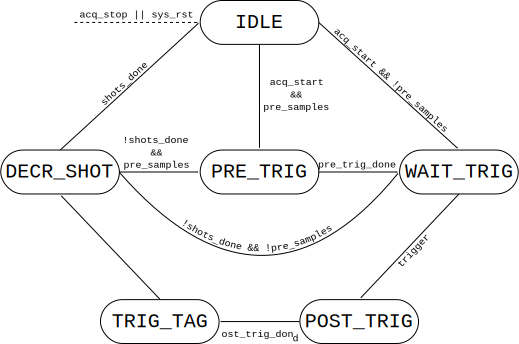
\includegraphics[width=0.8\textwidth]{figures/acq_fsm.pdf}}
            	\caption{Finite state machine of the acquisition}
            	\label{fig:acq_fsm}
            \end{figure}
            
            For the purpose of data acquisition, it implements the finite state machine, presented in Fig. \ref{fig:acq_fsm}. At start-up, the finite state machine is in IDLE state. After receiving the signal to start the acquisition, it starts acquiring data, which it writes to the memory using the Direct Memory Access (DMA), and waits for a trigger. After receiving the trigger it acquires the number of post-samples specified by the user. The acquisition is repeated until obtaining the requested number of acquisitions. After that, it returns the obtained data, enters the IDLE state and waits for the signal to start another acquisition \cite{fmc_adc_gateware_guide}. 
            The data written to the memory contains the samples from each channel and the information if the current sample is aligned with the trigger. The data is passed through the timestamping core, that allows determining the time of the trigger.
        
        \subsubsection{software}
            The FPGA resources are accessed by the ADC library, which makes use of the driver. The library provides a generic API for accessing the digitiser boards. It allows to:
            \begin{itemize}
                \item Configure the ADC parameters.
                \item Start the acquisition.
                \item Access the data, together with the information about the trigger and the timestamp.
            \end{itemize}

        
\section{White Rabbit Trigger Distribution} \label{section:WRTD}
    The key element of the DO is White Rabbit Trigger Distribution. It uses WR for clock synchronisation and exchanging data.
    %what is the goal
    \subsection{Purpose of WRTD} \label{subsec:purpose_of_wrtd}
        The purpose of WRTD is the ability to trigger the devices at the specified time. Depending on the application the requirements could be the following:
        \begin{itemize}
            \item Trigger the devices at exactly the same time.
            \item Trigger the devices with well specified delay between the triggers. 
        \end{itemize}
        Depending on the configuration, the WRTD can fulfil both of the requirements. 
    
    \subsection{Basic block of WRTD} \label{subsec:WRTD_block}
        %the building block
        The WRTD network is constructed of the basic building blocks, which share the same time reference determined by the 125~MHz clock of WR. The schematic of the WRTD block is depicted in Fig. \ref{fig:wrtd_block}.
        \begin{figure}
        	\centerline{\includegraphics[width=100mm]{figures/wrtd_block.pdf}}
        	\caption{Basic building block of the WRTD network}
        	\label{fig:wrtd_block}
        \end{figure}
        %local connections
        \textit{Local in} and \textit{Local out} are connections with devices to which there is a direct physical access. The devices that could be potentially connected are the following:
        \begin{itemize}
            \item Input devices:
            \begin{itemize}
                \item WRTD enabled ADC, generating the trigger when the measured value crosses the threshold voltage.
                \item Time to Digital Converter --- device that generates the timestamp at the time specified by the edge of the incoming pulse signal.
            \end{itemize}
            \item Output devices:
            \begin{itemize}
                \item WRTD enabled ADC, triggering on the time determined by the timestamp.
                \item Fine Delay --- device that generates the pulse at the time specified by the timestamp.
            \end{itemize}
        \end{itemize}
        %remote connections
        \textit{Remote in} and \textit{Remote out} are the connections with other WRTD blocks. Each output message from the connection that is not specified as local is sent over the network and could be used to trigger the devices connected to any of the other WRTD blocks. Each block could receive or discard the message depending on the rules set by the user, which will be described in the next sections.

    %API
    \subsection{WRTD API}
        The behaviour of the network is specified using the WRTD API. The structure and the functions available in the API were written in a way to be as compliant with LXI as possible. The available functions are listed in Tab. \ref{tab:wrtd_api}.
        
        The library contains the following types of functions:
        \begin{itemize}
            \item General --- initialisation, resetting and closing of the library as well as monitoring the internal state of the library
            \item Error handling
            \item Logs management
            \item Rules management --- the rules are responsible for interconnection of the blocks
            \item Alarms management --- alarms define at what time the event should be generated
            \item Attributes setters --- attributes modify the behaviour of the rules and the alarms
            \item Attributes getters
        \end{itemize}
        
        \begin{table}
\centering
\caption{List of the functions from the WRTD API}
\begin{tabular}{cc}
Type of function & Name of the function \\
\hline
\hline
\multirow{5}{*}{General} 
& wrtd\_init \\                                                                
& wrtd\_close \\                                                                  
& wrtd\_reset \\ 
& wrtd\_get\_sys\_time \\                                                      
& wrtd\_reset\_rule\_stats \\   
\hline
\multirow{2}{*}{Error handling} 
& wrtd\_get\_error \\                                                             
& wrtd\_error\_message \\  
\hline
\multirow{2}{*}{Logs management} 
& wrtd\_log\_read \\                                                           
& wrtd\_clear\_log \\ 
\hline
\multirow{5}{*}{Rules management} 
& wrtd\_add\_rule \\                                                           
& wrtd\_disable\_all\_rules \\                                                    
& wrtd\_remove\_rule \\                                                           
& wrtd\_remove\_all\_rules \\                                                     
& wrtd\_get\_rule\_id \\  
\hline
\multirow{5}{*}{Alarms management} 
& wrtd\_add\_alarm \\                                                          
& wrtd\_disable\_all\_alarms \\                                                
& wrtd\_remove\_alarm \\                                                       
& wrtd\_remove\_all\_alarms \\                                                 
& wrtd\_get\_alarm\_id \\ 
\hline
\multirow{5}{*}{Attributes setters} 
& wrtd\_set\_attr\_int32 \\                                                    
& wrtd\_set\_attr\_int64 \\                                                    
& wrtd\_set\_attr\_bool \\                                                     
& wrtd\_set\_attr\_tstamp \\                                                   
& wrtd\_set\_attr\_string \\   
\hline
\multirow{5}{*}{Attributes getters} 
& wrtd\_get\_attr\_int32 \\                                                       
& wrtd\_get\_attr\_int64 \\                                                    
& wrtd\_get\_attr\_bool \\                                                        
& wrtd\_get\_attr\_tstamp \\                                                      
& wrtd\_get\_attr\_string \\   
\end{tabular}
\label{tab:wrtd_api}
\end{table}
        
    \subsection{Example of usage}
        In order to explain how the library works, the example of the library configuration is presented. The examples fulfil the requirements specified in section \ref{subsec:purpose_of_wrtd}.
        
        \subsubsection{Fixed delay} \label{subsec:WRTD_fixed_delay}
            In order to be able to trigger one device with another with a fixed, well known delay, appropriate rules have to be set and configured. Each rule has 4 attributes:
            \begin{itemize}
                \item Source --- determines which event/device is the source of the trigger.
                \item Destination --- determines which device/connection should be triggered.
                \item Delay --- determines the amount of time that should be added to the timestamp.
                \item Enable --- determines if the given rule is enabled.
            \end{itemize}
            In order to connect two remote devices, two rules have to be established, with an example configuration presented in Tab. \ref{tab:wrtd_example}.
            
            \begin{table}
            \centering
            \caption{Example configuration to connect two devices using WRTD}
            \begin{tabular}{ccc}
            Attribute & Triggering device --- ADC1 & Triggered device --- ADC2 \\
            \hline
            Source & LC-I0 & LAN1 \\
            Destination & LAN1 & LC-O0 \\
            Delay & 500~ns & 0 \\
            Enable & 1 & 1 \\
            \end{tabular}
            \label{tab:wrtd_example}
            \end{table}
            
            The schematic of this connection are presented in Fig. \ref{fig:wrtd_connection}.
            
            \begin{figure}
            	\centerline{\includegraphics[width=\textwidth]{figures/wrtd_connection.pdf}}
            	\caption{Example of connectivity of two devices using WRTD}
            	\label{fig:wrtd_connection}
            \end{figure}
            
            An example code for the configuration of the rules for distribution and reception of the WRTD triggers are presented in Lis. \ref{cap:trig_dist} and Lis. \ref{cap:trig_rec} respectively.
            
            \begin{lstlisting}[style=CStyle, 
                   caption = Example configuration of the rule for distributing the WRTD triggers., 
                   label=cap:trig_dist]
const char * name = "trig_dist"                                                
enum wrtd_status status;                                                       
struct wrtd_dev *wrtd; //WRTD device returned by the wrtd_init                 
struct wrtd_tstamp ts;                                                         
ts.seconds = 0;                                                                
ts.ns = 500;                                                                   
ts.frac = 0;                                                                   
                                                                               
status = wrtd_add_rule(wrtd, name);                                            
WRTD_RETURN_IF_ERROR(status);                                                  
                                                                               
status = wrtd_set_attr_string(wrtd, name, WRTD_ATTR_RULE_SOURCE, LC-I0);          
WRTD_RETURN_IF_ERROR(status);                                                  
                                                                               
status = wrtd_set_attr_string(wrtd, name, WRTD_ATTR_RULE_DESTINATION, LAN1);   
WRTD_RETURN_IF_ERROR(status);                                                  
                                                                               
status = wrtd_set_attr_tstamp(wrtd, name, WRTD_ATTR_RULE_DELAY, &ts);          
WRTD_RETURN_IF_ERROR(status);                                                  
                                                                               
status = wrtd_set_attr_bool(wrtd, name, WRTD_ATTR_RULE_ENABLED, 1);            
WRTD_RETURN_IF_ERROR(status);   
\end{lstlisting}


\begin{lstlisting}[style=CStyle, 
                   caption = Example configuration of the rule for reception the WRTD triggers., 
                   label=cap:trig_rec]
const char * name = "trig_rec"                                                 
enum wrtd_status status;                                                          
struct wrtd_dev *wrtd; //WRTD device returned by the wrtd_init                    
struct wrtd_tstamp ts;                                                            
ts.seconds = 0;                                                                   
ts.ns = 0;                                                                        
ts.frac = 0;                                                                      
                                                                                  
status = wrtd_add_rule(wrtd, name);                                               
WRTD_RETURN_IF_ERROR(status);                                                     
                                                                                  
status = wrtd_set_attr_string(wrtd, name, WRTD_ATTR_RULE_SOURCE, LAN1);           
WRTD_RETURN_IF_ERROR(status);                                                     
                                                                                  
status = wrtd_set_attr_string(wrtd, name, WRTD_ATTR_RULE_DESTINATION, LC-O0);  
WRTD_RETURN_IF_ERROR(status);                                                     
                                                                                  
status = wrtd_set_attr_tstamp(wrtd, name, WRTD_ATTR_RULE_DELAY, &ts);             
WRTD_RETURN_IF_ERROR(status);                                                     
                                                                                  
status = wrtd_set_attr_bool(wrtd, name, WRTD_ATTR_RULE_ENABLED, 1);               
WRTD_RETURN_IF_ERROR(status);   
\end{lstlisting}

            
            LC-I0 means local input connection, LC-O0 means local output connection. With such a configuration, the triggering device will send a timestamp to the remote connection called LAN1, when there will be some event on its local connection. The value of the timestamp will be equal to the time when the event was produced, plus the time specified as the delay, in this case 500~ns. The triggered device will produce an event on its local connection at the time specified by the timestamp received on the LAN1 remote connection. In order to trigger the second device at the required time, the user has to make sure that the value of the delay is bigger than the worst-case delay of the network. The worst-case delay can be calculated based on the length of the cables that connect the devices in the WR Network and the delays of the particular elements of the network. 
        
        \subsubsection{Triggering at the same time}
            In order to trigger devices at a specified time, WRTD provides the functionality of alarms. The user can add an alarm that will trigger the devices at the specified time. Because of the common time reference, if various ADCs have the same value of the alarm, they will trigger at the same time.
            
    \subsection{implementation}
        In order to configure the WRTD, the FPGA resources have to be accessed. The access is provided by means of the mockturtle framework. 
        
        %mockturtle
        The essential components of this framework are the soft Central Processing Units (CPU) cores implemented in the FPGA. Each of the cores can run a different C application. In order for the soft CPU cores to communicate with the host machine, the mockturtle framework implements the mechanism of message queues. 
        
        WRTD implements a firmware for the mockturtle cores, in order to allow an access to the required FPGA cores \cite{mockturtle_ohwr}. The WRTD API is built on top of this firmware and hides the implementation details. The code that makes use of the API is run on the host machine. The user of the WRTD does not have to know anything about the mockturtle nor the firmware.
        
\section{Communication}
    In distributed systems, one of the main issues that have to be solved is to establish communication between the nodes. The problem is split into three parts:
    \begin{itemize}
        \item enumeration of the devices
        \item communication using Remote Procedure Calls (RPC)
        \item data transmission
    \end{itemize}
    The available technologies that may be used to solve the issues are presented in the following sections:
    
    \subsection{Enumeration of the devices} \label{subsec:zeroconf}
        %Problem description
        In distributed systems, one of the problems that have to be solved is how to detect available devices. 
        %First solution
        The common solution is to have a central unit, to which each new device connects when it is added to the network. For this, the devices have to be properly configured to know what the address of this central unit is. 
        
        %Second solution
        In order to avoid the necessity of manual configuration, many of the laboratory equipment use zeroconf networking. There exist various libraries for this purpose. In DO Python-Zeroconf~\cite{zeroconf} is used because it is the most common library in Python. 
        
        In Python-Zeroconf the server broadcasts the necessary information to create a connection: in the most basic case its IP address and the port on which it is listening. The device that appears in the network receives that information and automatically connects. The restriction of that technology is that it is limited to local networks.

    \subsection{Remote Procedure Call} \label{subsec:chap3:communication:rpc}
         RPCs allow executing the functions on remote clients. RPC eases the integration of applications, allowing invoking remote procedures as if they were local. However, it is important to distinguish if the call is local or remote because the RPC could be orders of magnitude slower than the local call, as well as less reliable. 
        
        It is typically implemented using a request-response messaging pattern. Applications that want to expose some functionalities provide a set of functions that can be executed, which is known by both the server and the client. The function that is executed on the server depends on the request of the client, which receives the result of the operation in the response.
        
        There is a great variety of available RPC libraries, among which the most common are:
        \begin{itemize}
            \item XML-RPC --- it is available in The Python Standard Library. It uses Extensible Markup Language (XML) for data transport, therefore it is not very efficient if a great amount of data should be sent between the client and the server.
            \item gRPC --- it is the RPC developed by Google. It is very efficient, yet more complicated to start using than the other libraries. It uses google protocol buffers for serialisation of data.
            \item RPyC --- it is a library mainly optimised for ease of use and "seamless RPC". It allows easy integration of applications, yet for an inexperienced user, it is not necessarily the best choice because it creates an illusion that there is no difference between the local and the remote call.
            \item own implementation --- RPC could be easily implemented using request-reply pattern with any type of transport, e.g. raw TCP or ZeroMQ. In some cases, this could be the best option, since the user can implement all the required features, without depending on the external library and without any overhead in the development time.
            %Probably in the implementation chapter write about the fact, explain that the RPC should not be complicated nor nested, because they could lead to blocking of the program, especially that it is more difficult to debug the problem if it is on two different machines. 
            %in the implementation chapter write what are the requirements, what did I try, how I did the final decision
        \end{itemize}
        For reasons presented in section \ref{section:rpc_selection}, own implementation of the RPC was chosen. After doing a series of measurements, presented in section \ref{section:data_transport_opt}, ZeroMQ library was chosen as a data transport.
    
    \subsection{Data transmission} \label{subsec:ZeroMQ}
        For data transmission, the ZeroMQ library was chosen. ZeroMQ is an open-source asynchronous messaging library. It is optimised mainly for high performance and low latency. It aims at large distributed systems, where the problem of scalability becomes an issue. The API is designed to resemble the Berkeley sockets. It implements various features that the developer would have to handle himself using the raw TCP. The key features are the following:
        \begin{itemize}
            \item The input/output operations are handled in background threads, using lock-free data structures, which allows scaling the applications easily. 
            \item It automatically queues the messages and provides the features to deal with high water marks. 
            \item The format of the messages is not imposed. It allows using the built-in serialiser, as well as to use any kind of the product on top.
            \item It automatically reconnects in case of lost connection and allows connection of the nodes in an arbitrary order.
            \item It allows establishing communication between the applications using arbitrary transports: TCP, inter-process or in-process.
        \end{itemize}
        ZeroMQ supports many messaging patterns, for which the library provides various types of sockets:
        \begin{itemize}
            \item REQ/REP --- they are meant for a simple synchronous request-reply pattern, where each request expects one reply.
            \item DEALER/ROUTER --- they extend the request-reply pattern allowing for an asynchronous operation.
            \item PUSH/PULL --- they are meant for distributing large amounts of data, in one direction.
            \item PUB/SUB --- they are used to distribute data in nodes arranged in the pipeline.
            \item RADIO/DISH --- they are used to distribute data from a single publisher to multiple subscribers
            \item CLIENT/SERVER --- they are used to create standard client-server applications, where the client initiates the conversation and the server can talk to one or multiple clients.
        \end{itemize}
        More advanced scenarios could be implemented using combinations of the described sockets \cite{zeromq_guide}.
        
    
    %In the optimisation and/or implementation : Do the measurements, compare it, chose the best solution, don't forget to take into account the simplicity of the solution, not only the efficiency
    \subsection{Serialisation} \label{subsec:serialisation}
        In distributed systems, the data sent between the nodes has to be converted into some format that is understandable by all the nodes. In the following section various data formats and serialisation libraries are presented: 
        
        \subsubsection{Pickle}
            Pickle is a Python native library that implements binary protocols for serialisation and deserialisation of data. It is intended only for Python. The obvious consequences are that it is not possible to share data with code that is written in a different language, yet it is well optimised for Python. The major difference between pickle and generic serialisation libraries is that it keeps track of the objects that were already serialised, avoiding serialising the same object twice. Since it is a binary protocol, it is not human readable \cite{pickle}.
        
        \subsubsection{JavaScript Object Notation (JSON)}
            JSON is a data-interchange format that is designed to be easy to read and write for humans, as well as easy to parse and generate for machines. The data is represented in text format. The JSON is language-independent \cite{json}.
        
        \subsubsection{Protocol Buffers}
            Protocol Buffers are a mechanism for serialising data. They allow users to define the data structures in .proto files, then, using the protocol buffer compiler, they generate the data access classes, which can be included in the code. Protocol Buffers separate the data representation and serialisation, making it both human readable as well as efficient. They are language-independent \cite{protobuf}.

\section{Qt} \label{section:qt}
    Qt is an open-source toolkit for creating Graphical User Interfaces. It provides an environment for quick development of applications called QtCreator. It uses an event-driven programming model for interaction with the user. It allows easy integration with other libraries, as well as the development of critical elements of the application without using Qt constructs. It is written in C++, but provides bindings for many different languages, including Python. 


\chapter{Conception of the DO}

The DO is a solution to the problem of distributed data acquisition. It takes advantage of the knowledge gathered by other people while creating distributed systems (chapter 2), and modern technologies which are currently available (chapter 3).
A deep study of existing solutions and a proper choice of the technologies are fundamental in achieving the goal of the distributed data acquisition in an efficient way.

In order to fulfil this goal, the following fundamental questions had to be answered:
\begin{itemize}
    \item How to make sure that the data from various devices corresponds to the same moment in time?
    \item What should the architecture of the system be?
    \item How to establish communication between the nodes?
\end{itemize}
These questions are answered in this chapter. The implementation details are described in the following chapter.

\section{Data synchronisation} \label{section:data_synchronisation}
    As it is explained in section \ref{section:WRTD}, WRTD allows distributing the triggers with known delay. However, even though the time of the trigger and the value of the delay are known, it does not mean that the devices are triggered at the same time. While acquiring the synchronised data, it is desirable that the data correspond to the same moment in time. In order to achieve this, DO uses the WRTD project to distribute the triggers, modifies the acquisition settings of the ADCs and processes the acquired data in order to align it.
    
    The idea of this operation is presented in Fig. \ref{fig:DO_pre_post}. Since the delay between the triggers of the ADCs is known, the acquired pre-samples and post-samples\footnote{The arrow of post-samples pointing to the left means the negative value of the post-samples, which in this situation specifies the number of samples that are NOT acquired before the trigger. In the actual hardware, it is not possible to set a negative value of post-samples, therefore it is set to 0 and the acquired data is truncated.} (the samples that are acquired before and after the trigger accordingly), could be configured to compensate for the delay between the triggers. 
    
    \begin{figure}
    	\centerline{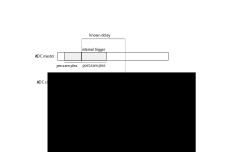
\includegraphics[width=0.7\textwidth]{figures/DO_pre_post.pdf}}
    	\caption{Configuration of pre-samples and post-samples in the DO}
    	\label{fig:DO_pre_post}
    \end{figure}
    
    In order to achieve this, two types of ADC configurations have been distinguished:
    \begin{itemize}
        \item master's ADC configuration --- the ADC which is triggered internally and distributes WRTD timestamps,
        \item slave's ADC configuration --- the ADC that is triggered by WRTD timestamps.
    \end{itemize}
    
    The user configures the master ADC the way he would configure a standard ADC, selecting the number of pre-samples and post-samples that he wants to acquire --- these values directly translate into the horizontal scale in the standard oscilloscope. 
    
    The slave ADCs have to be configured to return the data corresponding to the time of the trigger of the master ADC. For this purpose, the value of pre-samples and post-samples should be calculated according to the equations \ref{eq:pre-samples} and \ref{eq:post-samples}.
    
    \begin{equation}\label{eq:pre-samples}
        \text{pre-samples} = \text{pre-samples}_\text{required} + \Delta t * f_s
    \end{equation}
    
    \begin{equation} \label{eq:post-samples}
        \text{post-samples} = \text{post-samples}_\text{required} - \Delta t * f_s
    \end{equation}
    $\Delta t$ --- the known delay between the triggers,\\
    $f_s$ --- the sampling frequency of the ADC.
    
    With these settings, the number of samples that are acquired before and after the original trigger in each ADC is the same, therefore the data correspond to the same moment in time, even though the actual devices were triggered at different moments.
    
\section{General architecture} \label{section:general_architecture}
    When designing a distributed system, the question of architecture is fundamental. The choice of the architecture at the first phase of the project has a strong influence on all stages of the design, as well as the maintenance after deployment. That is why a lot of attention was devoted to this matter.
    
    There are two ways of connecting clients with each other. The first is to connect each device to each user, presented in Fig. \ref{fig:DO_schem_no_proxy}. The second option is to create a proxy that has the information about all the users and all the devices, presented in Fig. \ref{fig:DO_schem_proxy}. In the thesis, this proxy is called the DO Server. In case of using the term server e.g. in the RPC, it is explicitly stated. The Front End Computer (FEC) is a machine in which the ADC card is installed.

    \begin{figure}
    	\centerline{
\includegraphics[width=0.7\textwidth]{figures/DO_basic_schematics_no_proxy.pdf}}
    	\caption{Connection of clients and devices without proxy}
    	\label{fig:DO_schem_no_proxy}
    \end{figure}
    
    \begin{figure}
    	\centerline{
\includegraphics[width=0.7\textwidth]{figures/DO_basic_schematics.pdf}}
    	\caption{Connection of clients and devices using proxy}
    	\label{fig:DO_schem_proxy}
    \end{figure}
    
    The advantages of the design with the DO Server are the following:
    \begin{itemize}
        \item The system is divided into more smaller applications. It is easier to manage the code and upgrade its parts. However, the same result could be obtained designing the application properly in a modular way, yet for a inexperienced developer, such architecture enforces more careful design.
        \item In case of a design without the DO Server, some part of the code would have to be moved to the ADC application, which should be as lightweight as possible. The ADC application should be lightweight, because it may be run on a machine with little processing power, which serves uniquely as a host.
        \item In case of bigger networks, such a configuration is much easier to manage.
        \item If the DO is developed into a bigger system, the centralised unit having knowledge of all the connections could allow implementing algorithms optimising the access to the devices. However, at this moment, no such algorithm is implemented.
        \item The GUI module could be easily replaced with another application, not necessarily requiring plotting the data and having the graphical interface.
        \item Having a centralised unit eases the service discovery --- when adding a new device to the system, the address of just one element has to be known.
    \end{itemize}
    Counterarguments of using proxy are the following:
    \begin{itemize}
        \item Adding a proxy introduces some overhead in the communication between the user and the ADC.
        \item Adding a proxy introduces another abstraction layer, which could make the design unnecessarily more complicated in case of a small system. 
    \end{itemize}
    
    Taking into account all the arguments, the version with the DO Server was chosen. This choice has complicated the first stage of the design, however, the choice has proved to be good while testing the application and performing the measurements.
    
    The implementation details of various DO components are described in the following chapter.

\section{Communication} \label{section:communication}

    When designing a distributed system, apart from the general architecture, the other fundamental aspect is how the nodes communicate with each other. After analysis of the DO requirements, the following aspects of communication were pointed out:
    \begin{itemize}
        \item Enumeration of devices and establishing the connection. 
        \item Control of the run-time behaviour of nodes by the GUI.
        \item Transmission of the acquisition data and notifications.
    \end{itemize}
    The schematic of communication used in the DO is presented in Fig. \ref{fig:DO_communication}. The mentioned points are explained in more detail in the following sections.
    \begin{figure}
    	\centerline{
\includegraphics[width=\textwidth]{figures/DO_communication.pdf}}
    	\caption{Schematic of communication in the DO}
    	\label{fig:DO_communication}
    \end{figure}

    \subsection{Enumeration of the devices} \label{section:enumeration_of_devices}
        %Solution in DO
        %Introduction
        In order to ease the connection of new devices, it was decided that they should be discovered automatically by the DO Server. The other reason for this choice was to make the DO compatible with the LXI. The library chosen for that purpose was Python-Zeroconf, described in section~\ref{subsec:zeroconf}. Since there was no strict requirement for this particular technology, the choice of the library was based on its popularity.
        
        %How is it implemented
        The zeroconf listener runs on the DO Server. The ADCs, when connected to the network, advertise themselves. When the DO Server discovers a new device whose name suits the predefined restrictions, it starts the communication.
        
        This solution works correctly only as long as the devices are in the same local network. However, taking into account the fact that the DO is a distributed system, it cannot be assured that all the devices will be in the same local network. For this reason, two connection mechanism where implemented:
        \begin{itemize}
            \item Connection using zeroconf.
            \item Manual configuration.
        \end{itemize}
        If the server address is provided during the startup of the ADC application, the device connects to this address. Otherwise, it uses the previously described method.
    
    \subsection{Control of the run-time behaviour of the nodes} \label{section:run_time_beh}
        
        %reason for the RPC
        In order to control the run-time behaviour by the GUI, the RPC is used. This choice was made at the moment of selecting the architecture of the system: the main reason not to select the architecture with the DO Server was that it complicates the design. However, the use of the RPC was considered to make writing a distributed application in some way similar to writing a stand-alone application. Therefore, the choice of the architecture with the DO Server, together with the use of the RPC was considered the optimal solution, combining the advantages of the DO Server and reducing its greatest disadvantage --- the complexity.
        
        %data flow
        The distribution of the RPC servers and clients, presented in Fig. \ref{fig:DO_communication}, is based on the fact that the GUI is the node that controls the behaviour of the DO Server, and the DO Server controls the behaviour of the ADCs. There is no reason for the DO Server to issue an RPC to the GUI, therefore there is no RPC server in the GUI. The same applies for the ADC and the DO Server.
        
        At the beginning of the development of the DO, the communication scheme was not particularly well planned and the RPC servers were located in each of the nodes of the system. It caused issuing the nested RPCs, which at some point were blocking the entire application. This situation was a proof that the previous statement that \textit{the use of the RPC makes writing the distributed applications in some way similar to monolithic applications} was wrong.
        
        The implementation details and the choice of the RPC is described in more detail in the following chapter.
        
    \subsection{Transmission of acquired data and notifications} \label{section:transmission_data_notifications}
        RPCs are used for the majority of the communication between the modules except for three cases when there is an asynchronous event on the device side:
        \begin{itemize}
            \item acquired data
            \item notifications about the presence of the new device
            \item notifications about the availability of the device (in case it is used by different application)
        \end{itemize}
        
        When sending this information, there is no need for the callback, therefore one way communication is used. 
        For that purpose, the publisher/subscriber pattern is chosen, in which the publisher sends the asynchronous data to the subscriber. 
        
        In case of acquiring large arrays of data, this part of communication is the most crucial when optimising the speed of data acquisition. For that reason, various tools were evaluated in order to provide high speed and reliable data acquisition. The comparison of these tools is presented in section \ref{section:acquisition_speed_optimisation}.\\

    
    
    
     This chapter described the fundamental aspects considered when creating a system for a distributed data acquisition. The implementation details of the DO are described in the following chapter.


%Write why the Python in the next chapter.
%The core of the DO is the White Rabbit Trigger Distribution project, which allows the delivery of the timestamped events between %the devices. Internally, it uses the White Rabbit project for synchronisation and communication. In order to acquire and %imestamp the data, WR enabled digitizer board is used. At current state, only one board is supported ---FmcAdc100M14b4cha board %\cite{fmc_adc_ohwr}. In the future, support for other kinds of boards will be added. The DO itself is written in Python language, %using bindings to low level libraries. The technologies used in DO are presented in the following sections. 


%The idea of the DO is to allow to monitor the analog signals in the devices that could be located kilometers away from each other. In order to achieve this goal the DO uses the WRTD project, which allows distributing the triggers between the devices. The data is synchronised and sent to the final user. 


\chapter{Realisation of the DO}
The previous chapters describe the problem of the distributed data acquisition, the already existing solutions and how the DO approaches this problem and extends the previous concepts. In this chapter, the implementation of the DO is described in more detail.

For the implementation of the DO, the following work had to be done:
\begin{itemize}
    \item Deployment of the basic hardware setup, to demonstrate all of the crucial features of the system.
    \item Evaluation and selection of the most appropriate RPC.
    \item Implementation all the required applications:
    \begin{itemize}
        \item DO Server
        \item client applications:
        \begin{itemize}
            \item GUI
            \item test-bench
        \end{itemize}
        \item ADC application
    \end{itemize}
    \item Development of the design easy to test, debug and maintain afterwards.
    \item Development of the wrappers for the C libraries.
    \item Identification the issues of the WRTD.
    \item Optimisation the data transport.
    \item Optimisation the architecture.
\end{itemize}
All these issues are referred to in the following sections.

\section{Hardware setup and general concept} \label{section:hardware_setup}
    In order to demonstrate the crucial features of the DO, the setup presented in Fig.~\ref{fig:DO_hardware_setup}, Fig.~\ref{fig:DO_hardware_setup_photo} and Fig.~\ref{fig:DO_SPEC_FMC_front_panel} was deployed. The general concept of the DO is presented in Fig.~\ref{fig:DO_concept}.
    \begin{figure}
    	\centerline{
\includegraphics[width=\textwidth]{figures/DO_hardware_setup.pdf}}
    	\caption{The schematic of hardware setup of the DO}
    	\label{fig:DO_hardware_setup}
    \end{figure}
    \begin{figure}
    	\centerline{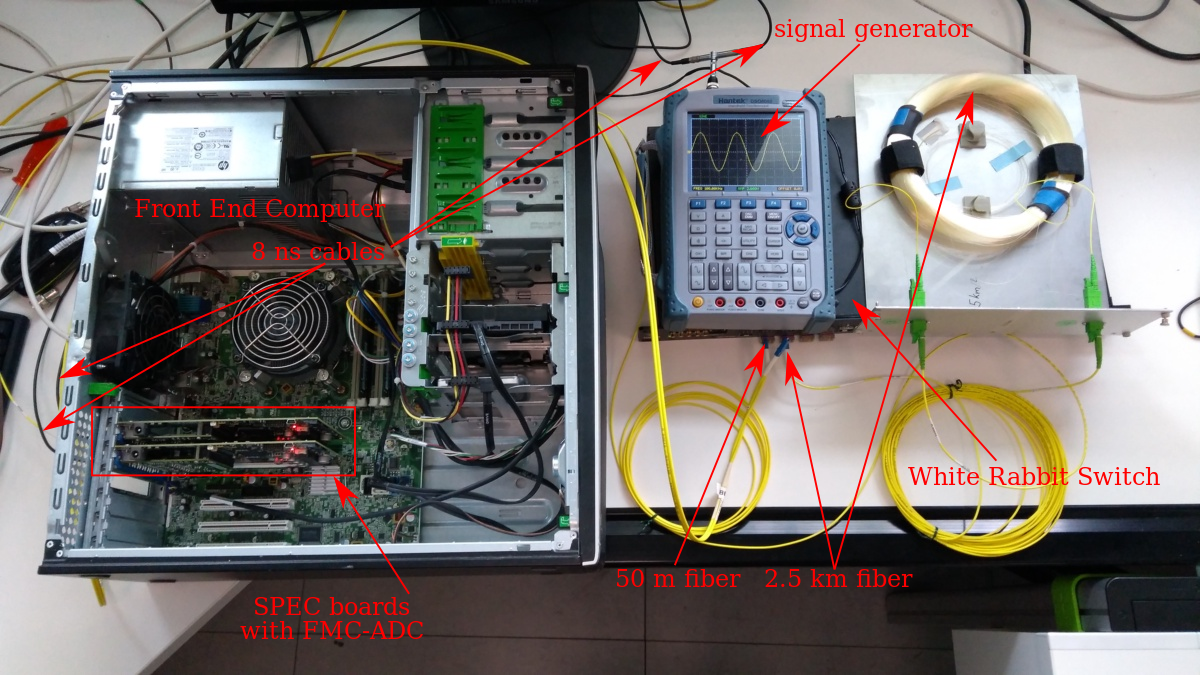
\includegraphics[width=\textwidth]{figures/DO_hardware_setup_photo.png}}
    	\caption{The photo of hardware setup of the DO}
    	\label{fig:DO_hardware_setup_photo}
    \end{figure}
    \begin{figure}
    	\centerline{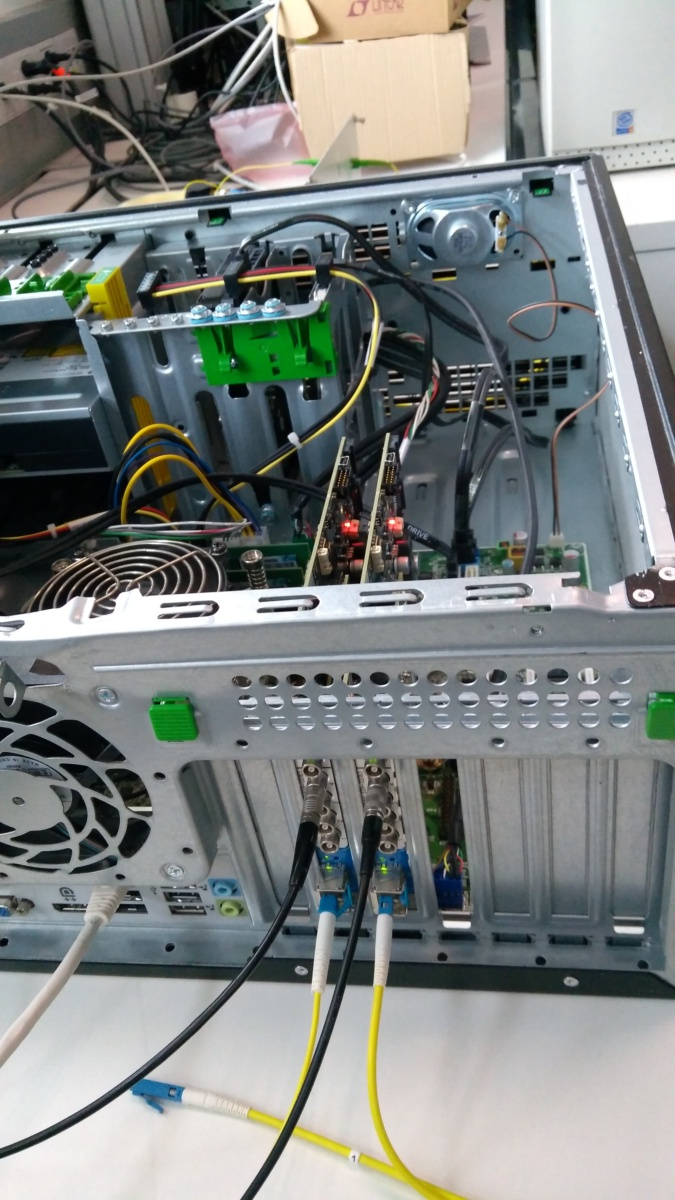
\includegraphics[width=0.6\textwidth]{figures/DO_SPEC_FMC_front_panel.jpg}}
    	\caption{The photo of the front panel of the SPEC board with FMC-ADC board}
    	\label{fig:DO_SPEC_FMC_front_panel}
    \end{figure}
    \begin{figure}
    	\centerline{
\includegraphics[width=\textwidth]{figures/DO_trigger_schem.pdf}}
    	\caption{The general concept of the DO}
    	\label{fig:DO_concept}
    \end{figure}
    
    In order to prove that the ADCs (section \ref{section:fmc_adc}) could acquire synchronised data independently of the distance, they were fed with the same sine signal and connected to the WR Switch (section \ref{section:WR}) with 50~m and 2.5~km fibres. Since both ADCs obtain exactly the same signal, measuring the phase shift between the obtained samples allows establishing the precision of the data synchronisation. Using fibre of a length in the range of kilometres allows simulating the synchronisation between the devices, whose distance is also in the range of kilometres. The schematic and photos depict the hardware setup and general conception of the DO. The software implementation details are presented in the next sections.


\section{RPC}   \label{section:rpc_selection}
    After implementation of the very first version of the DO and identification of the needs and the issues, the following list of requirements for the RPC was created:
    \begin{itemize}
        \item Transmission of synchronous messages --- this is the basic functionality of any RPC.
        \item Transmission of asynchronous messages --- it allows optimisation of the application.
        %\item Sending notifications --- in case at some point the communication scheme be changed and remove the publihser
        \item Polling on the connection --- it is common in many RPC libraries to create a separate thread for every connection. As described in section \ref{section:threads_management}, the DO is written with a minimum number of threads. For that reason, it was preferred to be able to poll on the connection and other file descriptors in the same thread, instead of adding new threads.
        \item Monitoring the state of the connection --- it allows detecting that the device was disconnected.
        \item It should use an efficient serialisation method or allow to serialise the data by an external library. It becomes important in case of sending large amounts of data. 
    \end{itemize}
    
    As the first approach, without yet having the requirements for the RPC, the XMLRPC was used. It was chosen mainly because it is very easy to deploy and it is in the Python Standard Library --- a smaller number of dependencies makes the project easier to maintain.
    After some time it was decided to look for another library because of the following reasons:
    \begin{itemize}
        \item It is not efficient. The reasons for the inefficiency are the following:
        \begin{itemize}
            \item It uses XML as the data format --- since it is a text format, unnecessarily big amounts of data are sent.
            \item It creates one connection per RPC instead of establishing a single communication channel.
        \end{itemize}
        \item It is impossible to send the dictionaries with integer keys: in the applications, the keys were converted into strings and then back to integers, only because of this restriction.
        \item It is impossible to send integers bigger than 24 bits --- bigger integers were split or converted to a string.
        \item It is not possible to monitor the state of the connection.
        \item Among all the previously mentioned requirements only two are satisfied, one of them partially:
        \begin{itemize}
            \item Transmission of synchronous messages.
            \item Polling on the connection --- it is possible only after modification of the source code of the XMLRPC server.
        \end{itemize}
    \end{itemize}
    
    After discovery of the problems with the XMLRPC, the previously mentioned list of the RPC requirements was created, to find the best solution. The following RPCs (described in section \ref{subsec:chap3:communication:rpc}) were taken into account:
    \begin{itemize}
        \item gRPC
        \item RPyC
        \item own implementation
    \end{itemize}
    
    None of the available libraries fulfils all the requirements. In the gRPC, it is impossible or difficult to monitor the state of the channel as well as there is no direct way to manually poll on the connection. In the RPyC there is no direct way to poll on the connection. 
    
    Finally, it was decided to use an own implementation of the RPC. It gives a lot of flexibility without or with very little of overhead in the development time. Most likely, if the custom implementation of the RPC was used straight away, it would have shortened the development time by avoiding the problems introduced by other libraries.
    
    %Choice of the transport
    It was decided to implement the RPC using ZeroMQ. The custom implementation of the RPC from now on will be called ZMQRPC. The other considered options were raw TCP sockets and another message queues. 
    
    %Why not TCP sockets
    The advantages of ZeroMQ sockets over raw TCP sockets are presented in section \ref{subsec:ZeroMQ}. The only advantage of the raw TCP sockets, in this case, is that it is easy to monitor the state of the TCP connection, while it is not the case for the ZeroMQ. The ZeroMQ provides an additional abstraction layer in order to provide reliable and robust transport of data, automatically reconnecting in case of lost connection. In many cases, it is desirable behaviour, but not in case of the DO. This problem could be overcome by adding timeouts when receiving the data from the sockets and implementing heart-beating. The heart-beating consists of periodically sending a message over the connection and in case of not receiving any reply for a predefined time, disconnecting the device. However, the heart-beating is not yet implemented in the DO.
    
    %Why not another message queues 
    Among other message queues libraries, the ZeroMQ was chosen based on the evaluation of various middle-ware products by the \textit{Software for Real-Time and Communication} group at CERN, presented in \cite{zmq_comparison} for the current equipment access framework \cite{zmq_icaleps}.
    
    The code for the basic RPC client is presented in Lis. \ref{cap:zmqrpc_client}
    
    \begin{lstlisting}[language=Python, 
                   caption = The code for basic RPC using ZeroMQ., 
                   label=cap:zmqrpc_client]
class ZMQ_RPC():                                                               
    def __init__(self, ip, port):                                              
        context = zmq.Context()                                                
        self.socket = context.socket(zmq.DEALER)                               
        self.socket.setsockopt(zmq.RCVTIMEO, 3000)                             
        addr = str(ip) + ':' + str(port)                                       
        self.socket.connect("tcp://" + addr)                                   
                                                                               
    def send_RPC(self, function_name, *args):                                  
        msg = [function_name, *args]                                           
        msg = pickle.dumps(msg)                                                
        self.socket.send(msg)                                                  
        try:                                                                   
            message = self.socket.recv()                                       
        except ZMQ_Timeout:                                                    
            logger.error("Server not replying")                                
            raise RPC_Error("Timeout of zmq socket.recv()")                    
            return None                                                        
        if message == b'Error':                                                
            logger.error(function_name + ' not available in the server')        
        else:                                                                  
            ret = pickle.loads(message)                                        
            logger.info(function_name + ' success')                            
            return ret  
\end{lstlisting}

    
    During the initialisation of the RPC client, the ZeroMQ socket is created, with a timeout equal to 3~s. The value of 3~s was selected in order not to block the program for too long in case of an error and not to be too short in case of any delay in the communication channel. In case of sockets where a delay in the communication channel is not expected, the value of the timeout is reduced. The socket connects to the server whose IP and port are provided. 
    
    The function responsible for executing the RPC, \textit{send\_RPC}, serialises the data, sends it through the socket and waits for the response. The response is returned to the caller.  
    
    The comparison of the XMLRPC server and ZMQRPC server is presented in Lis. \ref{cap:xmlrpc_server} and Lis. \ref{cap:zmqrpc_server} respectively. The code is practically the same. It consists of creation of a selector, registration of the server and polling on the file descriptor in the loop. Every time the poll returns, the call is executed.
    
    The reason for presenting these codes is to prove that custom implementation of the RPC does not introduce any overhead in the development time and is equally easy as using external library, giving at the same time more flexibility.
    
    \begin{lstlisting}[language=Python, 
                   caption = Examples code for XMLRPC server., 
                   label=cap:xmlrpc_server]
def run(self):    
    _ServerSelector = selectors.PollSelector                                   
    try:                                                                       
        with _ServerSelector() as selector:                                    
            selector.register(serv_expose.server, selectors.EVENT_READ)        
                                                                               
            while True:                                                        
                ready = selector.select(0.5)                                   
                if ready:                                                      
                    serv_expose.server._handle_request_noblock()               
                                                                               
                serv_expose.server.service_actions()                           
    finally:                                                                   
        pass 


\end{lstlisting}

    \begin{lstlisting}[language=Python, 
                   caption = Examples code for ZMQRPC server., 
                   label=cap:zmqrpc_server]
def run(self):                                                                 
    context = zmq.Context()                                                    
    socket = context.socket(zmq.ROUTER)                                        
    server_ip = get_ip()                                                       
    socket.bind("tcp://" + server_ip  + ":8003")                               
    poller = zmq.Poller()                                                      
    poller.register(socket, zmq.POLLIN | zmq.POLLERR)                          
                                                                               
    while True:                                                                
        socks = dict(poller.poll())                                            
        if socket in socks:                                                    
            [identity, message] = socket.recv_multipart()                      
            message = pickle.loads(message)                                    
            try:                                                               
                func = getattr(self, message[0])                               
                ret = func(*message[1:])                                       
                ret = pickle.dumps(ret)                                        
                socket.send_multipart([identity, ret])                         
            except AttributeError:                                             
                socket.send_multipart([identity, b"Error"]) 
\end{lstlisting}


    
    
\section{DO components} \label{section:do_components}

    \subsection{DO Server} \label{section:do_server_app}
        The DO Server is the central unit of the DO, responsible for management of the connections and for simple processing of data. 
        The simplified Unified Modeling Language (UML) class diagram of the DO Server application is presented in Fig.~\ref{fig:uml_server}.
        
        \begin{figure}
        	\centerline{
\includegraphics[width=\textwidth]{figures/UML_server.pdf}}
        	\caption{Simplified UML class diagram of the DO Server application}
        	\label{fig:uml_server}
        \end{figure}
        
        The DO Server consists of four major components:
        \begin{itemize}
            \item User class --- it is a model of the User application. In principle it is independent of the application, should it be GUI, test-bench or any other kind. It stands true under the assumption that each of the User applications behaves similarly to the classic oscilloscope, that is, it allows to connect the channels, select the trigger and collect the data. In case of any special requirements, more specified classes could inherit from the User class. Until now it was not necessary.
            \item ADC class --- it is a model of the connected device composed from the classes that represent particular functionalities of the ADC:
            \begin{itemize}
                \item Channel
                \item Trigger
                \begin{itemize}
                    \item Internal Trigger
                    \item External Trigger
                \end{itemize}
                \item Acquisition Configuration
            \end{itemize}
            %In the future, the models of the FDs and TDCs are going to be added.
            \item Connection Manager class --- it is responsible for registration and unregistration of the users and the devices as well as for providing the access to them for other classes.
        
            \item Communication --- in the DO Server there are four kinds of sockets used for communication with other applications:
            \begin{itemize}
                \item RPC client --- sends the RPC requests and receives the returned value.
                \item RPC server --- listens for the RPC requests, calls the respective function and sends back the returned value.
                \item Publisher --- sends the data without waiting for the reply.
                \item Subscriber --- receives the asynchronous data.
            \end{itemize}
            The sockets that are used to send data/requests, that is \textit{User publisher} and \textit{ADC RPC client}, are private to respective classes. The sockets that have to listen to asynchronous data, that is \textit{ADC subscriber}, \textit{User RPC Server} and \textit{Zeroconf Subscriber} are private to the \textit{Expose class}, that passes the data/requests to the \textit{Connection Manager} or to the respective \textit{Users} or \textit{ADCs}. The \textit{Expose class} implements a polling loop to listen on all of its sockets.
        \end{itemize}
        
        The following section describes the standard operation of the DO Server and its interactions with other applications.
        
        %Behaviour
        \subsubsection{Normal operation}
            The normal operation of the DO Server consists of five elements:
            \begin{itemize}
                \item Connections management --- The \textit{Expose} class listens for commands from Users applications, Device applications and Zeroconf to add or remove a service. Whenever the command is received, it is passed to the \textit{Connection Manager}, which creates or deletes respective User or ADC objects. In case of connecting or disconnecting the ADC, the notification is sent to the User that the device is available or unavailable. 
                
                \item User modification --- the User application can request to connect:
                \begin{itemize}
                    \item to the channel --- the User can connect to the channels of any of the ADCs that are not used by another User.
                    \item trigger --- the user can select either to trigger on the dedicated trigger input of any of the available ADCs or on the threshold of one of the connected channels. Only one trigger source can be selected. Whenever the trigger is selected, the master's configuration is assigned to the corresponding ADC and slave's configuration is assigned to the rest of the ADCs used by the particular user (see section~\ref{section:data_synchronisation}). The WRTD is configured to receive the timestamps from the master ADC and to distribute them to the slave ADCs. The slave ADCs are configured to trigger on the respective WRTD events.
                \end{itemize}
                
                \item ADC modification --- when the User application wants to modify the ADC configuration, it sends a message to the DO Server. The message contains the name of the ADC together with the name and the value of the parameter to configure. The request is pre-processed and respective commands are sent to the ADC application. Since the ADC application accesses the real hardware, in order to make sure that there was no error during the hardware access, the configuration of the ADC is retrieved after each request to modify any of the parameters. 
                
                \item Acquisition --- just like in a normal oscilloscope there are two acquisition modes:
                \begin{itemize}
                    \item single --- in this mode the acquisition of the ADC is configured once. When available, the data is received from the ADC application and sent to the User application. 
                    \item run --- in this mode the acquisition is configured in the loop, in order to obtain the data continuously. The detailed description of the acquisition loop is described in section \ref{section:acquisition_loop_opt}
                \end{itemize}
            \end{itemize}
            
    \subsection{GUI} \label{section:do_gui_app}
        %goal
        The GUI provides easy remote access to the connected devices in order to modify their configurations, collect the data and display it. 
        
        %first approach
        In the first approach to design the GUI, all possible configurations of the ADCs were exposed. A screenshot of the application with two ADCs connected is presented in Fig. \ref{fig:gui_first_approach}.

        \begin{sidewaysfigure}
        	\centerline{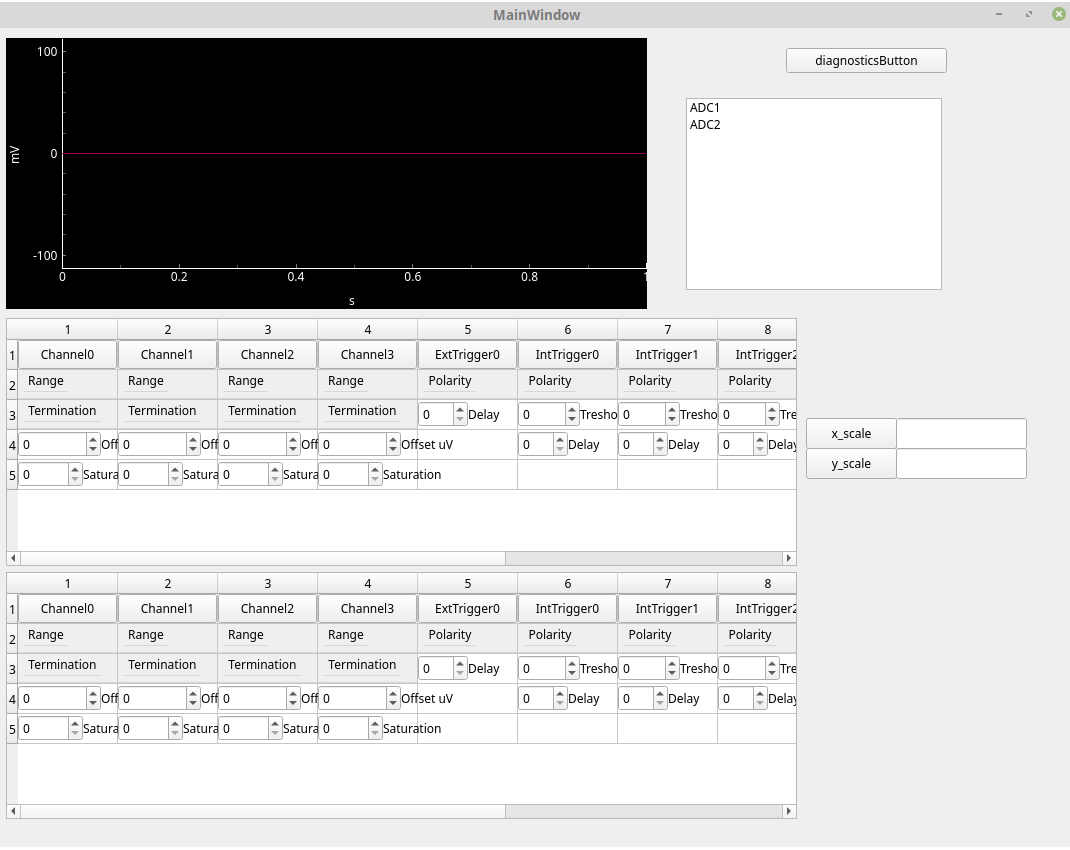
\includegraphics[width=0.9\textwidth]{figures/GUI_first_approach.jpg}}
        	\caption{The first version of the GUI}
        	\label{fig:gui_first_approach}
        \end{sidewaysfigure}
        
        It was a good starting point, which allowed to easily debug all the applications, but it turned out that in this way managing the synchronisation of the boards was more difficult. In order to configure the WRTD, the proper configuration of the triggers is necessary. Therefore there were two options:
        \begin{itemize}
            \item Allow the user to configure all the triggers.
            \item Hide some of the functionalities.
        \end{itemize}
        %why second approcah
        Since from the beginning of the project it was assumed that the synchronisation details should be hidden from the user, the second option was chosen. The updated version of the GUI is presented in Fig. \ref{fig:gui_current}.
        
        \begin{sidewaysfigure}
        	\centerline{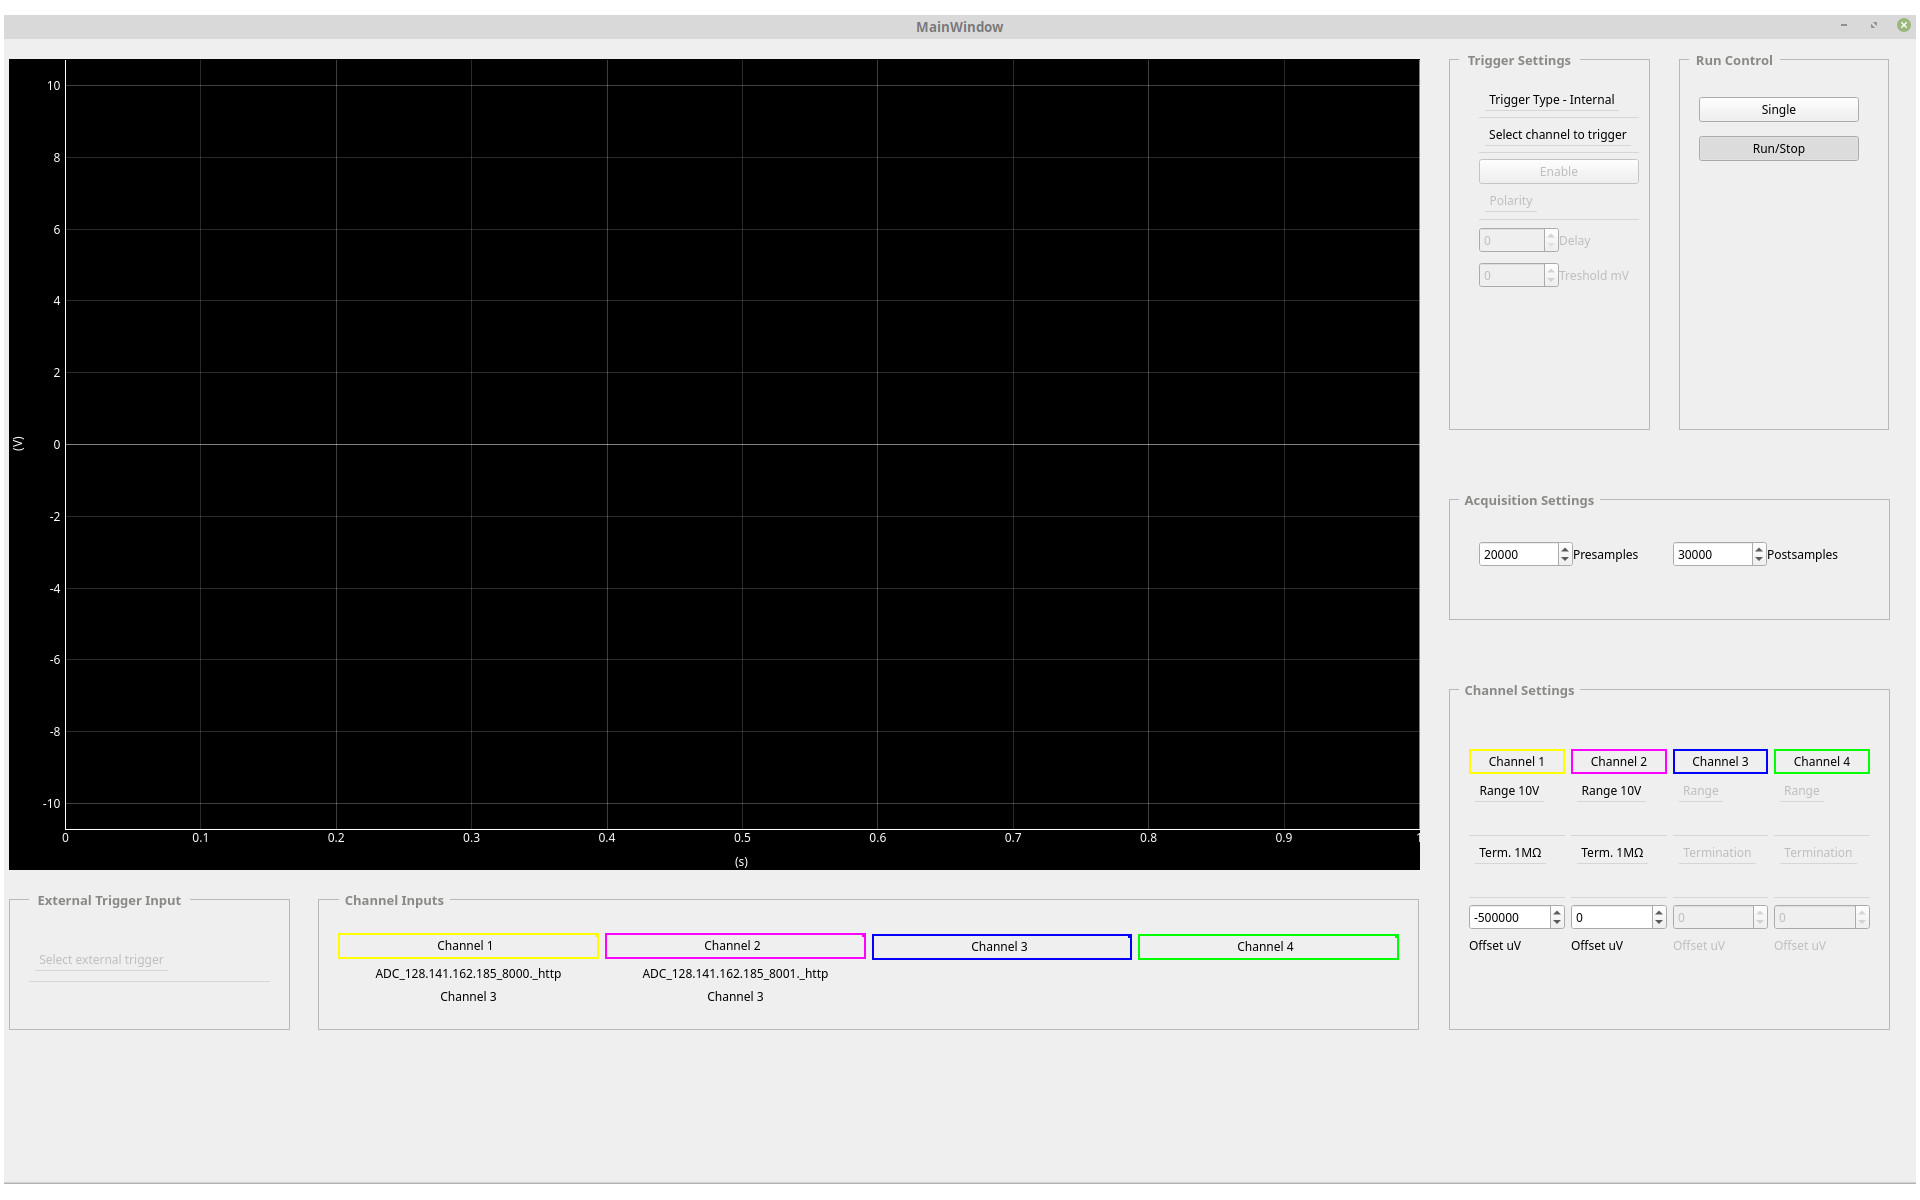
\includegraphics[width=\textwidth]{figures/GUI_current.jpg}}
        	\caption{The current version of the GUI}
        	\label{fig:gui_current}
        \end{sidewaysfigure}
        
        The design of the GUI was made as similar to the classical oscilloscope as possible. A special effort was made to make it intuitive, so that every electronics engineer could start using it just like every other oscilloscope.
        By now, it seems that this goal has been achieved partially. Taking into account the fact that the DO inevitably differs from a classical oscilloscope and there was not enough time to implement all the features of an oscilloscope, usually, some amount of explanation is needed for every new user.
        
        %design of the GUI
        Taking into account the chosen architecture (see section \ref{section:general_architecture}), it was assumed that the GUI should not process the data if it is not necessary and should only serve the three following functionalities:
        \begin{itemize}
            \item Allow the modification of the ADCs' parameters.
            \item Display the configuration of the ADCs.
            \item Display the acquired data.
        \end{itemize}
        The structure of the GUI application, presented in Fig. \ref{fig:gui_structure}, is straightforward. It is composed of various groups of settings of the oscilloscope and of the plot. Each group is composed of Qt widgets that have two functions:
        \begin{itemize}
            \item They represent the state of the setting they refer to.
            \item When the user modifies the widget, e.g. clicks on it, changes the value of the box etc., the widget invokes the function that is bound to it. The bound function, in the majority of cases, sends the information to the DO Server about the change of its state, using the RPC.
        \end{itemize}
        
        The \textit{server expose} module implements a polling loop to listen for the acquisition data and notifications about availability of the ADCs. Whenever any event is received, it uses the \textit{QT signals and slots mechanism} to transmit the data to the GUI.
        
        \begin{figure}
        	\centerline{
\includegraphics[width=0.7\textwidth]{figures/GUI_schematics.pdf}}
        	\caption{Simplified GUI application diagram}
        	\label{fig:gui_structure}
        \end{figure}
    
    \subsection{ADC} \label{section:do_adc_app}
        The structure of the ADC application is presented in Fig. \ref{fig:adc_structure}.
        \begin{figure}
        	\centerline{
\includegraphics[width=0.9\textwidth]{figures/ADC_schematics.pdf}}
        	\caption{Simplified ADC application diagram}
            	\label{fig:adc_structure}
        \end{figure}
        
        The purpose of the ADC application is to allow to remotely access the hardware resources:
        \begin{itemize}
            \item the ADC board
            \item the WRTD module
        \end{itemize}
        
        The ADC and the WRTD modules have full access to all of the hardware functionalities. However, for the purpose of the DO, direct access to the following functionalities is hidden:
        \begin{itemize}
            \item All of the WRTD functionalities.
            \item Pre-samples and post-samples modification --- the DO Server can select the value of the pre-samples and post-samples that it wants to receive, which does not always reflect the actual value used by the hardware (see section~\ref{section:data_synchronisation}).
        \end{itemize}
        The DO Server can select if the particular ADC works as the master or the slave in the network (see section~\ref{section:data_synchronisation}). With that information, the Device Access module appropriately configures the number of pre-samples and post-samples as well as it enables/disables necessary WRTD rules. 
        The rest of the ADC functionalities is exposed to the DO Server:
        \begin{itemize}
            \item Configuration of the ADC parameters.
            \item Retrieval of the configuration.
            \item Start/stop of the acquisition.
        \end{itemize}
        The communication with the DO Server is provided by the following modules:
        \begin{itemize}
            \item Zeroconf --- if the address of the DO Server is not known, Zeroconf notifies the DO Server about the presence of the new device.
            \item Publisher --- it publishes the acquired data. If the server address is known, it sends a notification about the presence of the new device to the DO Server.
            \item RPC server --- it provides remote access to the functionalities exposed by the Device Access. 
        \end{itemize}
        
        The libraries used to access the ADC board and the WRTD are written in C language. In order to ease the integration of the devices in the DO, Python wrappers were developed for both of these libraries. In order to directly access the C functions, the Python ctypes \cite{ctypes} library was used. The wrappers provide access to most of the functions provided by the libraries, except for the functions responsible for memory management, which is done automatically using Pythons constructors and destructors. The C specific parts of the library are hidden from the user.

    \subsection{Test-bench} \label{section:do_testbench_app}
        In order to provide a high quality code, a set of tests was developed.
        
        The most crucial elements of the DO are located in the DO Server and the ADC application. The GUI is responsible mainly to display the data and send the configuration. Therefore, taking into account the difficulty of writing the tests for graphical interfaces, it was decided to provide a script for testing the DO Server and the ADC. The features of the GUI are tested manually.
        
        The test script, which makes use of the Python unittest framework \cite{python_unittest}, replaces the GUI. Since the interface of the DO Server is generic, it is possible to connect various types of applications, including test-benches.
        
        The test script starts the DO Server application and the ADC applications. When the system is set, the test-bench connects to the DO Server as the User. Next, it sends the commands, reads back the configuration and compares if the data is coherent. Moreover, it provides the functionalities of measuring the acquisition time and frequency as well as the precision of the synchronisation. These functionalities were used to perform the measurements for this thesis.

\section{Threads management} \label{section:threads_management}
    The multi-threaded applications are desirable in case of systems that should be easily scalable. In a well-designed multi-threaded application, the processing capability increases with the number of processor cores. The main restriction that has to be taken into account is that the threads shouldn't access the same resources \cite{zeromq_guide}.
    
    The Python threads are not executed on different CPUs, so the code is not executed truly in parallel. These threads are generally used in cases when the code execution involves some waiting. That's why it seemed quite natural to use it for communication and data acquisition in the DO. During the development of the project, it was decided to minimise the number of threads because of the following reasons:
    \begin{itemize}
        \item The objects cannot be shared between the threads.
        \item To establish communication between the threads, the message queues have to be implemented. The functions that receive the data from the message queues are blocking, so adding such thread adds another level of abstraction without eliminating the problem.
        \item It is more difficult to debug the multi-threaded application.
        \item In case of wrong usage of mutexes it is easy to block the execution of the program.
    \end{itemize}
    
    If the execution of the program requires waiting for some resources, the alternative for using multiple threads is to use a single thread to poll on all of the resources in the loop and serve all of the requests. It avoids the problem of concurrent accesses and is much easier to debug. This approach is used in DO. However, additional threads were created in three cases:
    \begin{itemize}
        \item The GUI is run in the main thread, which is blocked after the start of the graphical interface. In order to receive the asynchronous data from the DO Server, using the non-QT library, it was necessary to implement a polling loop in the separate thread. The communication between the threads makes use of the \textit{QT signals and slots mechanism} \cite{qt_signals_slots}.
        \item The zeroconf service browser --- it uses one thread to listen for connections. Probably it would be possible to modify the code to poll on the file descriptor, but since it is a module with a very specific task, without any influence on the performance, it was decided to implement the message queue between the threads. For that purpose, the inter-process sockets are used.
        \item The test code starts the applications in different threads and uses the message queue to collect data from them.
    \end{itemize}
    The minimisation of the number of threads made the design much easier to test, debug and maintain afterwards.

\section{WRTD issues} \label{section:wrtd_issues}
The DO was the first user of the WRTD project before the release. One of the goals of the DO was to help to identify the issues of the WRTD before the release. Indeed, during the development of the project, the following issues were identified:
\begin{itemize}
    \item Single start of the acquisition was causing continuous acquisitions and flooding of the network with the timestamps.
    \item The timestamps were sent after the acquisition, not after receiving the trigger, which was causing the necessity of increasing the timestamp delay when increasing the number of acquired post-samples.
    \item Common bugs in the drivers and libraries of the ADC and WRTD --- eg. overflow etc.
    \item Wrong timing constraints of the HDL design that were causing communication errors.
    \item Issues with the ADC calibration.
    \item Issues with the acquisition of large numbers of samples.
\end{itemize}

Fast identification of the issues led to improvement of the tools.

    
\section{Acquisition speed optimisation} \label{section:acquisition_speed_optimisation}
    The amount of data that could be analysed in the distributed system depends on the acquisition frequency.
    In case of collecting data by the GUI in order to display it to the user, there is no point in increasing the frequency above what could be perceived by the human eye. 
    However, the data, instead of being plotted in the GUI, could be analysed to extract some information. In that case, there is no threshold frequency above which increasing it doesn't make sense. The data analysis, in the future, could be performed in the GUI. What is more, as it was mentioned in section \ref{section:general_architecture}, there are various types of applications that could be connected instead of the GUI, e.g. PMU. Therefore, it is important to increase the frequency of the acquisition. In order to achieve that, two parts of the code were optimised:
    \begin{itemize}
        \item The data transport
        \item The acquisition loop
    \end{itemize}
    
    \subsection{Optimisation of the data transport} \label{section:data_transport_opt}
        The time required to send the data between the clients is an important factor that could limit the acquisition frequency in the distributed system. In order to optimise this factor, the following transport methods were compared:
        \begin{itemize}
            \item XMLRPC --- it was the library that was initially used for the data transport.\footnote{In the initial version of the DO, the acquisition data was sent using the RPC. Afterwards, it was decided to keep the data transport and the RPC separate.}
            \item ZeroMQ --- the RPC used in the project uses ZeroMQ sockets. Therefore, it was considered reasonable to use the same library for the data transport, especially considering that the literature research showed this particular library to be well optimised \cite{zmq_comparison}.
            \item TCP --- the communication libraries usually use the TCP as the low level data transport. Therefore, the custom implementation of the communication using TCP sockets is also compared.
        \end{itemize}
        
        Since the data sent over ZeroMQ sockets and TCP sockets could be serialised by any kind of library and XMLRPC is limited to the XML, which is the text format, it was expected that XMLRPC would have much worse performance. The comparison between ZeroMQ and TCP was more important, since it was not certain if ZeroMQ is well optimised and would improve the time of the data transport or if it introduces unnecessary overhead, slowing down the connection.
        
        In order to compare the methods, the acquisition time between the moment of sending the command to start the acquisition and receiving the data from one ADC was measured. The ADC was configured to trigger internally. The measured signal was a sine wave of frequency 100~kHz --- the time between starting the acquisition and receiving the trigger is negligible. The serialisation method used for the ZeroMQ and the TCP was Pickle (see section \ref{subsec:serialisation}) --- the Python standard serialisation package. In case of XMLRPC, it was obviously XML. The acquisition time was measured for various numbers of post-samples per channel, from four channels. Each of the measurements was repeated 5 times and the medium value was calculated. All the results are presented in both linear and logarithmic scale. The vertical lines represent the standard deviation, however sometimes the value of the standard deviation is so small that it is not visible in the plot.
        
        Fig.~\ref{fig:meas:xml_zmq_tcp_comp_pikle} presents the comparison of the acquisition speed while using three of the previously mentioned methods. Since the data corresponding to the ZeroMQ and TCP cannot be differentiated in the figure, Fig.~\ref{fig:meas:zmq_tcp_comp_pikle} presents the comparison of just these two methods. 
        All results are very similar for a small number of samples, that is up to 1000. Differences are visible for greater numbers of samples. The presented figures clearly show that, as it was expected, the XMLRPC's performance is the worst. The result of the ZeroMQ and the TCP are very similar, therefore both of them were included for further evaluation.
        
        \begin{figure}
            \centering
            \begin{minipage}[b]{0.8\textwidth}
                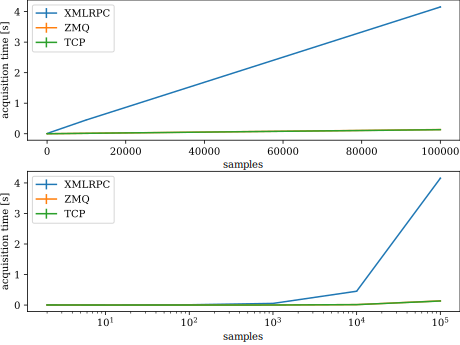
\includegraphics[width=\textwidth]{figures/measurements/xml_zmq_tcp_comparison_pickle.pdf}
            	\caption{Comparison of the acquisition speed using XMLRPC, ZeroMQ and TCP}
                \label{fig:meas:xml_zmq_tcp_comp_pikle}
            \end{minipage}
            \vfill
            \vspace{1cm}
            \begin{minipage}[b]{0.8\textwidth}
                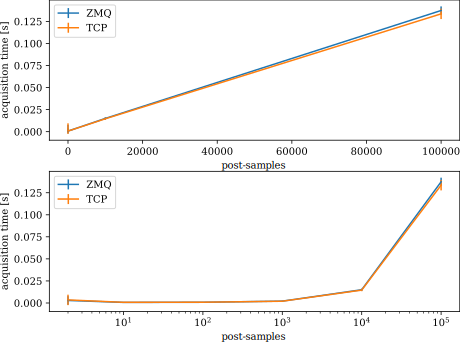
\includegraphics[width=\textwidth]{figures/measurements/zmq_tcp_comparison_pickle.pdf}
            	\caption{Comparison of the acquisition speed using ZeroMQ and TCP}
                \label{fig:meas:zmq_tcp_comp_pikle}
            \end{minipage}
        \end{figure}
        
        As the next step, three serialisation methods were compared (the serialisation libraries are described in section~\ref{subsec:serialisation}):
        \begin{itemize}
            \item Pickle,
            \item JSON,
            \item Protocol Buffers.
        \end{itemize}
        
        The measurements were done using both kinds of sockets: ZeroMQ and TCP. The results are presented in Fig. \ref{fig:meas:ser_comp_zmq} and Fig. \ref{fig:meas:ser_comp_tcp}.
        
        \begin{figure}
            \centering
            \begin{minipage}[b]{0.8\textwidth}
            	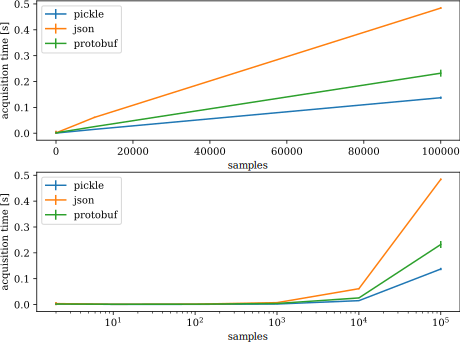
\includegraphics[width=\textwidth]{figures/measurements/zmq_serialization_comp.pdf}
            	\caption{Comparison of the serialisation libraries using ZeroMQ}
            	\label{fig:meas:ser_comp_zmq}
            \end{minipage}
            \vfill
            \vspace{1cm}
            \begin{minipage}[b]{0.8\textwidth}
            	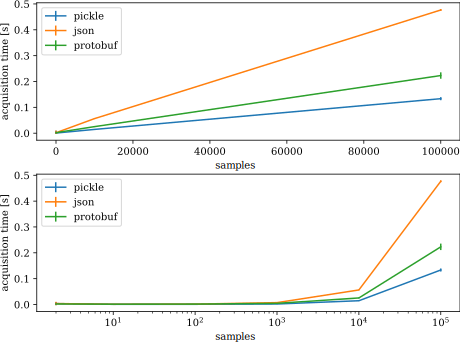
\includegraphics[width=\textwidth]{figures/measurements/tcp_serialization_comp.pdf}
            	\caption{Comparison of the serialisation libraries using TCP}
            	\label{fig:meas:ser_comp_tcp}
            \end{minipage}
        \end{figure}

        Clearly, in both cases the best result are obtained using Pickle as the serialisation library, therefore this library is used for all of the following measurements.
         
        Since the results obtained using ZeroMQ and TCP are very similar, even though TCP has slightly better performance, it ZeroMQ is used in the project, in order not to introduce too many technologies and for being consistent with the technology used for the RPC. The added value of the performance's increase would not be enough to compensate for the complication of the project.
        
        While optimising the acquisition loop, presented in the following section, another part of the code was also optimised. The acquired raw data had to be converted to volts. Before, each sample was converted in the standard Python loop. Since this part of code was introducing big delays, the Numpy \cite{numpy} library was used to convert the data. This optimisation resulted in significant increase of the acquisition speed. In order to be able to compare the following optimisation with previous results, the measurements were repeated, with the optimised convertion method. Otherwise, it would not be clear if the increase in performance was caused by a different conversion method or by acquisition speed optimisation. Moreover, it was desired to make sure that with this optimisation, there still would not be a great difference between the ZeroMQ and the TCP. The results are presented in Fig.~\ref{fig:meas:zmq_tcp_comp_pikle_numpy}. 
        
        \begin{figure}
        	\centerline{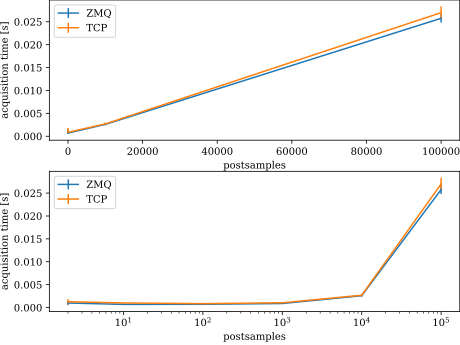
\includegraphics[width=0.8\textwidth]{figures/measurements/zmq_tcp_comparison_pickle_numpy.pdf}}
        	\caption{Comparison of the acquisition speed using ZeroMQ and TCP after code optimisations}
            	\label{fig:meas:zmq_tcp_comp_pikle_numpy}
        \end{figure}
        
        The increase of the acquisition speed when compared to the previous results was significant. However, the difference between the ZeroMQ and the TCP remained small. Therefore, all other measurements were performed using ZeroMQ sockets.
        
    \subsection{Optimisation of the acquisition loop} \label{section:acquisition_loop_opt}
        In the first approach,  when the DO Server was receiving a command to start a continuous acquisition from a particular GUI, it was configuring all the necessary ADCs to start a single acquisition. The ADC with a master configuration (see~section~\ref{section:data_synchronisation}) was configured at the and to make sure that the WRTD timestamps would be distributed only after all the other ADCs were already configured. The DO Server, after receiving the data from all required ADCs, was processing the data and sending it to the GUI. After that, the procedure was repeated. In this approach, the acquisition loop was situated in the DO Server.
        
        In the second approach, when the DO Server is receiving a command to start a continuous acquisition from a particular GUI, it is configuring the ADCs to start a continuous acquisition. The received data from all of the ADCs is buffered. After receiving the data from all the required ADCs, with corresponding timestamps, the data is sent to the GUI. In this approach, the acquisition loop is situated in the ADC.
        
        The simplified DO Server's state machines diagrams for both approaches are presented in Fig.~\ref{fig:loop_server_fsm} and Fig.~\ref{fig:loop_adc_fsm}.
        
        \begin{figure}
            \centering
            \begin{minipage}[b]{0.45\textwidth}
            	
\includegraphics[width=\textwidth]{figures/loop_server_fsm.pdf}
            	\caption{The simplified state machine in the DO Server --- the acquisition loop in the DO Server}
                \label{fig:loop_server_fsm}
            \end{minipage}
            \hfill
            \begin{minipage}[b]{0.45\textwidth}
            	
\includegraphics[width=\textwidth]{figures/loop_adc_fsm.pdf}
            	\caption{The simplified state machine in the DO Server --- the acquisition loop in the ADC}
                \label{fig:loop_adc_fsm}
            \end{minipage}

        \end{figure}
        
        The first approach was easier to implement, since it was much easier to debug. The ease of debugging was caused by the following reasons:
        \begin{itemize}
            \item The timestamps were distributed only after all of the ADCs were already configured. Therefore, the issues caused by trying to trigger a not configured ADC did not have to be taken into account.
            \item The successive data would not arrive into the DO Server before the previous one was already processed. Therefore, any errors could be immediately detected. When the problem occurred, the DO Server application was not flooded with the consecutive data. Moreover, when the DO Server was processing the data too slow it was not causing any error --- the only effect was that the acquisition frequency was getting lower.
        \end{itemize}
        
        Even though the approach with the acquisition loop in the DO Server was easier to implement, it was decided to move the acquisition loop to the ADC, since a significant increase in the performance was expected.
        
        In order to compare the performance of both approaches, the acquisition frequency for various numbers of pre-samples was measured. The configuration of the boards was exactly the same as the one described in section~\ref{section:data_transport_opt}.
        
        The acquisition frequency was calculated based on the number of data packets received from from the DO Server, during 0.5~s, calculated from the moment of sending the request to start a continuous acquisition. Each measurement was repeated 5 times. The results are presented in Fig. \ref{fig:meas:loop_adc_server_comp}. The plots represent the medium value, the vertical lines the standard deviation. 
        
        \begin{figure}
        	\centerline{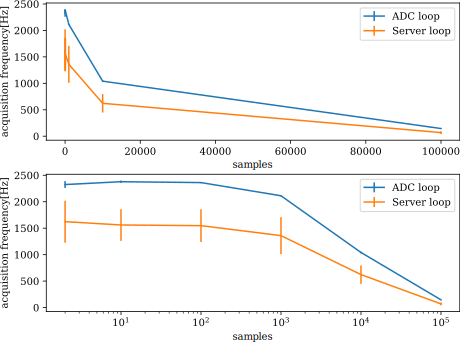
\includegraphics[width=0.8\textwidth]{figures/measurements/loop_adc_server_comparison.pdf}}
        	\caption{Comparison of the acquisition frequency when the acquisition loop is placed in the DO Server and in the ADC}
            	\label{fig:meas:loop_adc_server_comp}
        \end{figure}
        
        From the presented measurements it is clear that the optimisation of the acquisition loop increased the performance of the system significantly. It is worth noting, that the approach with the acquisition loop in the DO Server has much bigger variance. It is caused by the fact that in this approach the frequency depends on a bigger number of factors --- more commands are exchanged between the DO Server and the ADC. Therefore, there is a greater probability that a latency in the communication channel would occur.
        
\section{Measurements of the precision of the synchronisation} \label{section:precision_measurements}
    When acquiring the data synchronously, one of the most important parameters is the precision of the data synchronisation. In the DO the precision depends on the precision of timestamping of the acquired signal and on the precision of the timestamping clock. The timestamping clock is the WR clock, whose accuracy is of 1~ns (section \ref{section:WR}). Taking into account the fact that the timestamping clock (period 8~ns) is not locked to the sampling clock (10~ns period), the precision of the timestamping is of 10~ns. Therefore, the expected precision of the data synchronisation is of 11~ns.
    Another factor that has to be taken into account is that, because of ongoing modification of the hardware development conventions, there is no access to the EEPROM chip which stores the calibration data of the ADC, therefore the used ADCs are not calibrated.
    
    The signals are provided to the ADCs over 8~ns cables. However, the precision of the cables measurement is not known. In order to identify the errors introduced by the cables, all the precision measurements are repeated, switching the cables.
    
    The precision of the DO was measured using the setup presented in section \ref{section:hardware_setup}.
    The accuracy is measured as a distance of the zero-crosses between the measured signals from the two ADCs. The precision is calculated as 3$\sigma$ value of the normal distribution fitted to the measured data. The first ADC is triggered internally, the other by the timestamp from the previous one. The zero-cross is defined as a value for which a linear function is zero. The linear function is defined by two points: the last point whose value is negative and the first point whose value is positive. The measured signal was a square wave of frequency 1~kHz.
    
    The distance was measured 20000 times. The histograms of the measurements are presented in Fig. \ref{fig:meas:wrtd} and in Fig. \ref{fig:meas:wrtd_sig_rev}.
    
    \begin{figure}
        \centering
        \begin{minipage}[b]{0.8\textwidth}
        	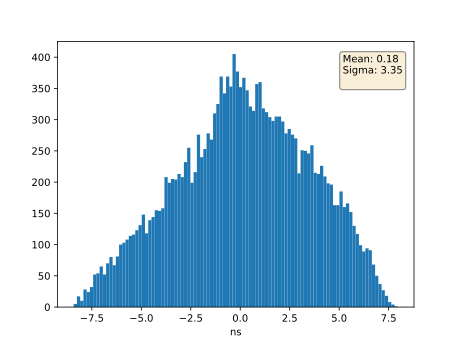
\includegraphics[width=\textwidth]{figures/measurements/WRTD.pdf}
        	\caption{The histogram of the accuracy of the data synchronisation.}
            \label{fig:meas:wrtd}
        \end{minipage}
        \vfill
        \vspace{0.5cm}
        \begin{minipage}[b]{0.8\textwidth}
        	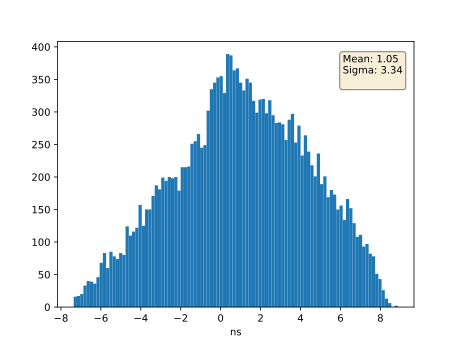
\includegraphics[width=\textwidth]{figures/measurements/WRTD_sig_rev.pdf}
        	\caption{The histogram of the accuracy of the data synchronisation, cables reversed.}
            \label{fig:meas:wrtd_sig_rev}
        \end{minipage}
    \end{figure}
    
    
    The results are very close to the expected ones: the mean value is equal 0.18~ns in the first configuration of the cables and 1.05~ns in the second configuration. Therefore, the difference between the cables lengths, measured in time of the signal propagation, is $ (1.05\:ns - 0.18\:ns)/2 = 0.44\:ns$. 
    As a proof that the lack of calibration could be the result of the mean value different from 0, the measurement was repeated, with the offset of the signal optimised to minimise the absolute value of the distance between the zero-crosses. The results are presented in Fig. \ref{fig:meas:wrtd_calib}. The shape of the distribution remains the same, only the mean value is moved to zero. 
    
    \begin{figure}
    	\centerline{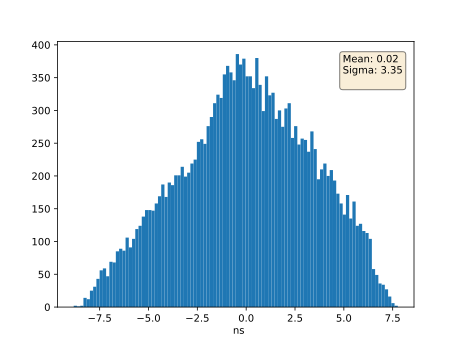
\includegraphics[width=0.8\textwidth]{figures/measurements/WRTD_calibration.pdf}}
        	\caption{The histogram of the accuracy of the data synchronisation, offset optimised.}
            \label{fig:meas:wrtd_calib}
    \end{figure}
    
    The value of 3$\sigma$ is equal to 10~ns. This result is slightly better than the expected one of 11~ns. 


    However, it must be stated, that the mean of the distribution can vary with time. Fig. \ref{fig:meas:wrtd_other_day} presents the same measurements taken another day. 
    \begin{figure}
    	\centerline{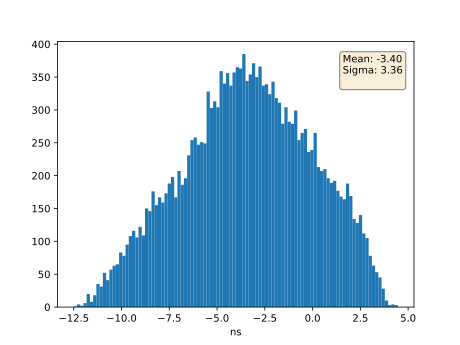
\includegraphics[width=0.8\textwidth]{figures/measurements/WRTD_other_day.pdf}}
        	\caption{The histogram of the accuracy of the data synchronisation taken another day.}
            \label{fig:meas:wrtd_other_day}
    \end{figure}
    The histogram shape remains the same, however the mean value is different. This behaviour could be partially caused by temperature differences of the board, which could explain differences in the range of few hundreds pico-seconds. Other sources of such behaviour should be investigated in the future work.

\chapter{Conclusion and future work}

The Distributed Oscilloscope is an outcome of the work done by the author of this thesis in collaboration with Hardware and Timing section, Controls group, Beams department at CERN.

The DO consists of various applications (section \ref{section:do_components}), which together allow monitoring the signals from various digitisers, located far away from each other. In order to perform the measurements, the digitisers used during the development are installed in the same PC. However, in order to simulate the distance between them, the devices are synchronised over a 2.5~km optical fibre (section \ref{section:hardware_setup}). 

The DO uses the WRTD project for synchronisation of devices, distribution of timestamps and triggering devices based on the value of timestamps received from other devices (section \ref{section:WRTD}). The precision of the synchronisation, calculated as 3$\sigma$ value of normal distribution fitted to the measurements of the synchronisation accuracy (section \ref{section:precision_measurements}), is equal to 10 ns, which is better than the assumed precision: $\pm (T_s + 1~ns = 11~ns)$ \footnote{The frequency of the sampling clock is 100 Mhz. Therefore the sampling period ($T_s$) is equal to 10 ns}, subject to the mean variation caveat mentioned in section \ref{section:precision_measurements}.

The DO project is available as a Python module, published on the OHWR page \cite{distributed_oscilloscope} together with the documentation, which provides the details on installation and usage. In order to provide a user-friendly interface a GUI application was written (section \ref{section:do_gui_app}). It allows configuration of devices and displaying the acquired data. All the synchronisation details are implemented in the Server (section \ref{section:do_server_app}) and in the ADC application (section \ref{section:do_gui_app}), and are hidden from the user. 

Development of the DO allowed to identify and solve a lot of WRTD issues before its first release (section \ref{section:wrtd_issues}).

Based on the presented results, the goal (section \ref{section:goal}) of the thesis has been achieved, meeting the above mentioned requirements.


\section{Contributions made in this thesis}
The DO uses a variety of projects which are currently internal to CERN or which are published in Open Hardware Repository (OHWR) \cite{ohwr}. The list of contributions made by the author in this thesis is presented below:
\begin{itemize}
    \item Development of the following applications of the Distributed Oscilloscope:
        \begin{itemize}
            \item Distributed Oscilloscope Server (section \ref{section:do_server_app})
            \item Distributed Oscilloscope GUI (section \ref{section:do_gui_app})
            \item Distributed Oscilloscope ADC (section \ref{section:do_adc_app})
            \item Distributed Oscilloscope Test-bench (section \ref{section:do_testbench_app})
        \end{itemize}
    \item Implementation of Python wrappers for C libraries (section \ref{section:do_adc_app})
    \item Investigation of various design aspects of the distributed system:
        \begin{itemize}
            \item General architecture (section \ref{section:general_architecture})
            \item Communication (section \ref{section:communication}):
                \begin{itemize}
                    \item Enumeration of devices (section \ref{section:enumeration_of_devices})
                    \item Control of run-time behaviour of nodes:
                        \begin{itemize}
                            \item Selection of the method (section \ref{section:run_time_beh})
                            \item Comparison of various RPC libraries and implementation of custom RPC (section \ref{section:rpc_selection})
                        \end{itemize}
                    \item Transmission of acquired data and notifications \ref{section:transmission_data_notifications})
                \end{itemize}
            \item Threads management (section \ref{section:threads_management})
        \end{itemize}
    \item Building the hardware setup (section \ref{section:hardware_setup})
    \item Debugging WRTD and solving minor issues (section \ref{section:wrtd_issues})
    \item Optimisation of the acquisition speed:
        \begin{itemize}
            \item Optimisation of the data transport (section \ref{section:acquisition_speed_optimisation})
            \item Optimisation of the acquisition loop (section \ref{section:acquisition_loop_opt})
        \end{itemize}
    \item Performing measurements of the precision of the DO (section \ref{section:precision_measurements})
\end{itemize}


\section{Future work}
The following list presents the scope for further work:
\begin{itemize}

    \item Improving the precision of data synchronisation
    
    Currently, the greatest source of synchronisation errors is the fact, that the acquisition clock is not locked to the timestamping clock. What is more, these clocks have different frequencies. However, it is possible to exchange the ADC chip in FMC-ADC board (section \ref{section:fmc_adc}), to the one that would work with the same frequency as the timestamping clock. After this change, the HDL design would have to be modified, to lock the acquisition clock to timestamping clock. The expected precision after these changes is  $\pm~1~ns$.
    \item Improving the time stability of the accuracy of data synchronisation
    
    The mean value variations in time, presented in section \ref{section:precision_measurements} should be investigated. The source of this variations should be eliminated.
    \item Adding support for different types of devices
    
    Currently, the only available device that could be connected in the DO is the FMC-ADC board (section \ref{section:fmc_adc}). In the future, support for different ADCs, as well as different types of devices should be added.
    \item Adding different types of User Applications
    
    Currently, there are two User Applications available: GUI and test-bench. In the future, depending on users requirements, other applications could be added. 
    
    \item Heart-beating
    
    Heart-beating, described in section \ref{section:rpc_selection}, could be implemented in order to reliably detect the disconnection of a device.
\end{itemize}

\vfill % otherwise Latex tries to fill up all the page

%check the UML diagram                                                       


\begin{singlespace}  % use single-line spacing for multi-line text within a single reference
	\setlength\bibitemsep{\baselineskip}  %manually set separataion betwen items in bibliography to double space
	\printbibliography[title={References}]
\end{singlespace}

\addcontentsline{toc}{chapter}{References}  %add References section to Table of Contents

\pagebreak
\begin{acronym}[OASIS] % Give the longest label here so that the list is nicely aligned
\acro{OASIS}{Open Analogue Signal Information System} % +
\acro{CERN}{The European Organization for Nuclear Research} % +
\acro{LIST}{LHC Instability Trigger Distribution project} % +
\acro{LHC}{Large Hadron Collider} % +
\acro{WR}{White Rabbit} % +
\acro{LXI}{LAN eXtensions for Instrumentation} % +
\acro{DO}{Distributed Oscilloscope} % +
\acro{WRTD}{White Rabbit Trigger Distribution} % +
\acro{API}{Application Programming Interface} % +
\acro{PCIe}{Peripheral Component Interconnect Express} % +
\acro{GUI}{Graphical User Interface} % +
\acro{PMU}{Phase Measurement Unit} % +
\acro{PTP}{Precision Time Protocol}
\acro{DMA}{Direct Memory Access}
\acro{ADC}{Analogue to Digital Converter}
\acro{CPU}{Central Processing Unit}
\acro{RPC}{Remote Procedure Call}
\acro{XML}{Extensible Markup Language}
\acro{UML}{Unified Modeling Language}
\acro{SPEC}{Simple PCIe FMC carrier}
\acro{FMC}{FPGA Mezzanine Card}
\acro{FPGA}{Field-Programmable Gate Array}
\acro{FEC}{Front End Computer}
\acro{SFP}{Small Formfactor Pluggable}
\acro{DAC}{Digital to Analog Converter}
\acro{JSON}{JavaScript Object Notation}
\acro{OHWR}{Open Hardware Repository}

\acro{IVI}{Interchangeable Virtual Instruments}
\acro{LAN}{Local Area Network}


\end{acronym}
\listoffigures
\listoftables


\end{document}


